\documentclass[font=default]{mpltx}
\usepackage{bm, ctex, array}
\usepackage{subfigure, graphicx}
\usepackage{multirow}
% 以下至 \begin{document} 都仅是本文件为了方便额外定义的命令, 写报告时不需要.
\hypersetup{colorlinks=false}% 超链接带颜色
\usepackage{xcolor}
% 以上是本文件为了方便额外定义的命令, 写报告时不需要.
\linespread{1.5}
\begin{document}

\title{非线性热对流斑图} % 切合报告内容, 简短明确, 可以不同于讲义
\author{MaskedName} % 这里 \emailphone 一定要紧跟在 \author 后方
\emailphone{MyMail@stu.pku.edu.cn}{Tel}
% 如果改用 \email 则仅需要邮箱参数
\affiliation{北京大学物理学院\quad 学号: StudentID}
\date{\zhdate{2024/12/12}}

\begin{abstract}
  系统从无序到有序的转变一直以来是热力学以及非线性动力学前沿的研究方向。本实验通过搭建非线性热对流斑图的实验装置,观察了瑞利-贝纳德对流现象的产生、发展和演化过程。具体来说,实验中通过控制2mm、4mm薄层水的上下表面温差,实现了远离平衡态的开放系统从无序到有序的自组织转变过程,并通过阴影法将水的折射率分布进行可视化,观察非线性对流的特征。
\end{abstract}
\keywords{瑞利-贝纳德对流,非线性对流斑图,耗散结构理论,阴影法}

\maketitle

\section{引言}
热力学第二定律告诉我们,一个封闭的热力学系统总是由有序的状态向无序的状态进行演化。而在现实生活中,我们见到的更多的是开放系统。在开放系统中会出现丰富的自组织现象,即由局部的相互作用,从无序的状态向有序的状态进行演化。常见的例子有热对流结构、生命过程(如生物种群的进化过程)、化学振荡(如碘钟反应)等。这样从无序到有序的演化与系统的自发对称性破缺有关,而正是对称性的破缺才让我们的世界如此丰富多彩。

人们一直以来都想找寻一个同样的理论描述上述的自组织现象,而耗散结构理论就是其中的一个重要理论。耗散结构理论是由普利高津(Prigogine)在上世纪60年代提出的,它认为开放系统在远离平衡态时,会不断地和外界进行物质和能量的交换,在系统内部的某个参量达到一个阈值的时候,系统就有可能脱离原先无序的热力学分支,进而突变到一个全新的稳定的有序状态。由于这个过程中需要不断的与外界交换物质和能量,因此这种结构被称为耗散结构,耗散在这一过程中起到了非常重要的作用。

之后人们也在动力学的角度研究了这种自组织现象。动力学上的解释是:在系统的非线性效应很小的时候,系统内部出现的随机涨落会指数衰减,系统不会偏离原来的无序态。但是如果系统中的某个参数达到临界值,系统中出现的随机涨落会被逐渐放大,那么系统就会脱离原来的无序态,演化到一个新的稳定的耗散结构。

本实验观察的瑞利-贝纳德对流(Rayleigh-Bénard convection)正是耗散结构的一个典型例子。这是1900年贝纳德观察到的一个对流现象,后来瑞利对其做了详细的理论分析。当薄液体层上下温度差达到一个临界值的时候,就会出现对流现象,通过阴影法可以观察到对流斑图的形成和演化。而当温差过大的时候,稳定的耗散结构就会被湍流所替代,系统的演化变得不可预测。本实验通过观察对流斑图,研究了瑞利-贝纳德对流的特征,并且探讨了非线性对流的产生和演化过程。
\section{理论}
对于上下温度不同的两个无限大平板之间的热对流系统,我们可以使用纳维-斯托克斯(Navier-Stokes,简写NS)方程进行分析。我们的做法是对定态解加定向微扰,讨论微扰的线性发展。《近代物理实验》中已经给出去量纲化后关于微扰满足的方程组,这里不再赘述。方程组中一个重要的无量纲参数就是瑞利(Rayleigh)数:
\begin{equation}
    Ra=\frac{g\alpha d^3\Delta T}{\kappa\gamma}\propto d^3\Delta T.
\end{equation}
其中$\alpha,\gamma,\kappa$分别为流体的热膨胀系数、粘度和热导率,$d$为流体层的厚度,$\Delta T$为上下温度差,$g$为重力加速度。线性稳定性分析方法是将微扰方程中的所有变量看作小量,忽略非线性项。如果我们假设有$z$方向的初始微扰$u_z$:
\begin{equation}
    u_z=A(z)e^{i(k_xx+k_yy)+st},\quad |k|=\sqrt{k_x^2+k_y^2}=\alpha.
\end{equation}
求解结果中要看$s$的实数部分正负号如何,若$s$的实数部分为负,则微扰随时间衰减,原定态解稳定;若$s$的实数部分为正,则微扰随时间越来越大,原定态解不稳定。

对于微扰方程组来说,$Ra$是一个可变参数,和温度差成正比。在实验中我们知道温度差较低时,均匀态(无序态)稳定,而温度差较高时,均匀态不稳定。而从稳定到不稳定的过程中有一个临界值,通过线性稳定性分析可以求得这个临界值,详细推导过程在这里不做详述,这里指给出瑞利数的临界值:
\begin{equation}
    R_c\approx 1707.76.
\end{equation}
\begin{figure}
    \centering
    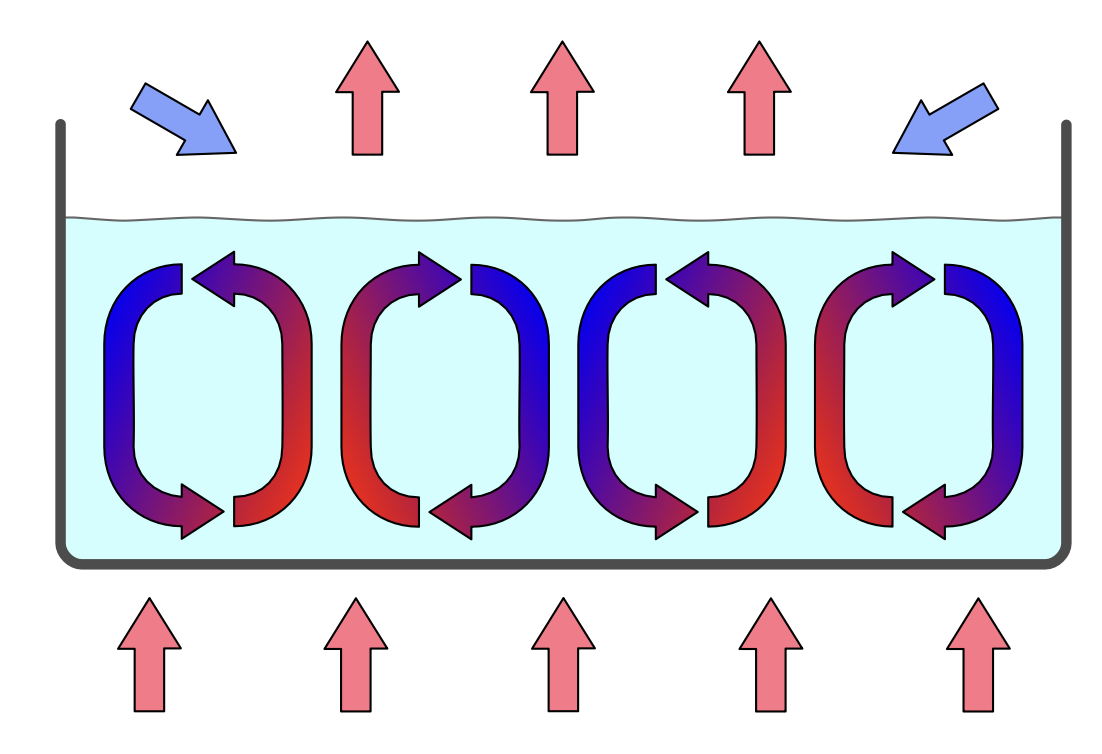
\includegraphics[width=0.55\textwidth]{fig/convection.png}
    \caption{瑞利-贝纳德对流示意图}
    \label{fig:convection}
\end{figure}

当$Ra<R_c$时,系统中随机出现的扰动噪声会随时间衰减,以保持定态解的稳定性。而当$Ra>R_c$时,满足条件的的部分扰动噪声就会随时间放大,非线性项将发挥重大作用。常用的方法是多尺度分析,可得扰动振幅满足的非线性方程,这里不做详细推导。而由于非线性项的贡献,系统会形成稳定的对流斑图,如\autoref{fig:convection} 所示。但是当$Ra$过大时,系统会失去稳定,进入湍流状态。
\section{实验内容}
\begin{figure}
    \centering
    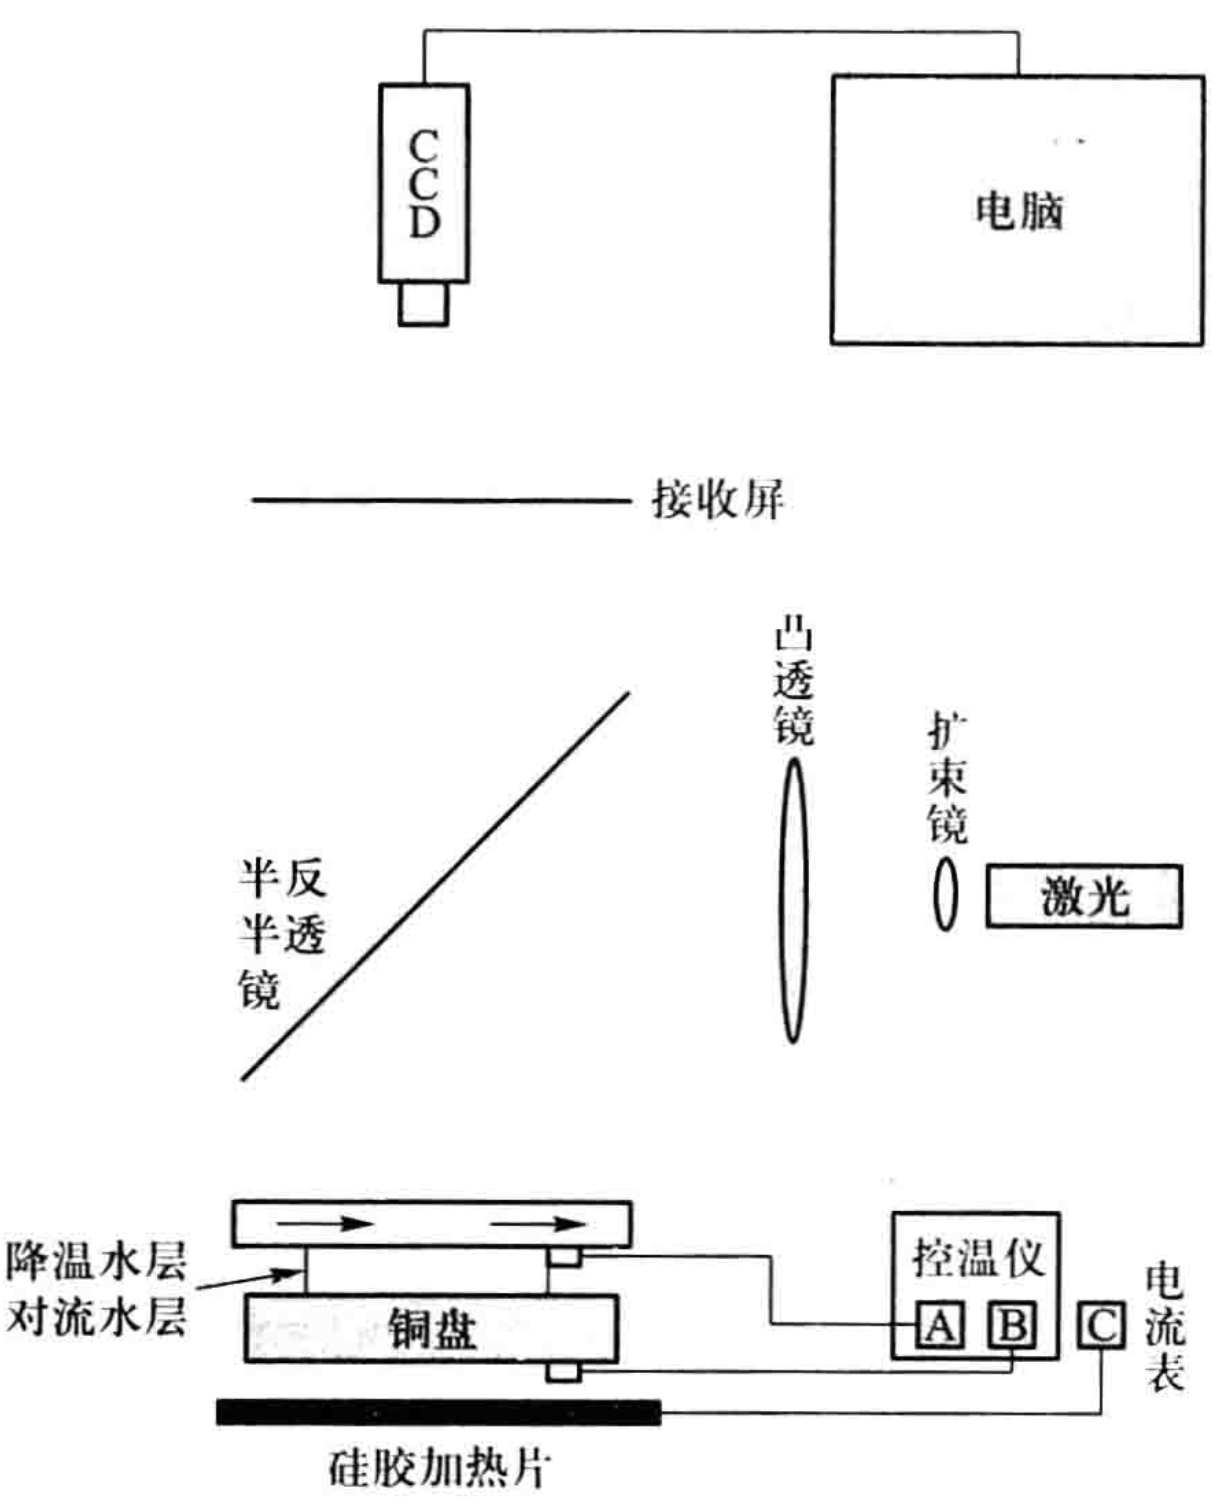
\includegraphics[width=0.45\textwidth]{fig/setup.png}
    \caption{实验装置示意图}
    \label{fig:setup}
\end{figure}
本实验的实验装置如\autoref{fig:setup} 所示。对流层的上、下表面分别使用纯净的蓝宝石和镀金的黄铜,这两种材料相对于水有高出两个量级的热导率,这保证了温度在边界上能够均匀分布。上表面使用水冷降温,底面使用硅胶片进行加热。激光通过对流水层后在金膜反射后打在接收屏上,并通过CCD进行数字成像。

上面用光学成像反映水层折射率变化的方法称作阴影法。我们简单将折射率分布不均匀的水层看作透镜,当流场中的$\partial^2 n/\partial y^2$不等于常数的时候,不同位置的光线会被聚焦到不同的位置,从而在接收屏上形成明暗不同的斑图。具体来说,成像的亮区对应冷水下降区域,暗区对应热水上升区域,具体分析见思考题。

具体实验步骤如下:
\begin{enumerate}
    \item 调整激光光路,使得CCD成像区域中心被均匀照亮。
    \item 选取$d=2$ mm的黑色环,将环方于铜盘和蓝宝石之间,并在其中加入水,形成2 mm的水层。静置30 min至1 h,使水层进入稳定的平衡状态。
    \item 调整硅胶加热片的电流,待水层温度差稳定之后(一般调电流之后10 min即可达到新的稳定状态),观察CCD成像。
    \item 调整不同的温度差成像,寻找系统从无序到有序的临界点,并观察斑图的变化。
    \item 将水层厚度调整为$d=4$ mm,重复上述步骤,观察斑图的变化。
\end{enumerate}

\section{实验结果与分析}
用CCD拍摄到的部分实验结果如\autoref{fig:convection_photos_2mm} 和\autoref{fig:convection_photos_4mm} 所示,加热电流$I$和温差$\Delta T$标记在每张图的下侧。
\begin{figure}
    \centering
    \subfigure[$I=0.40$ A, $\Delta T=2.7\ ^\circ\text{C}$]{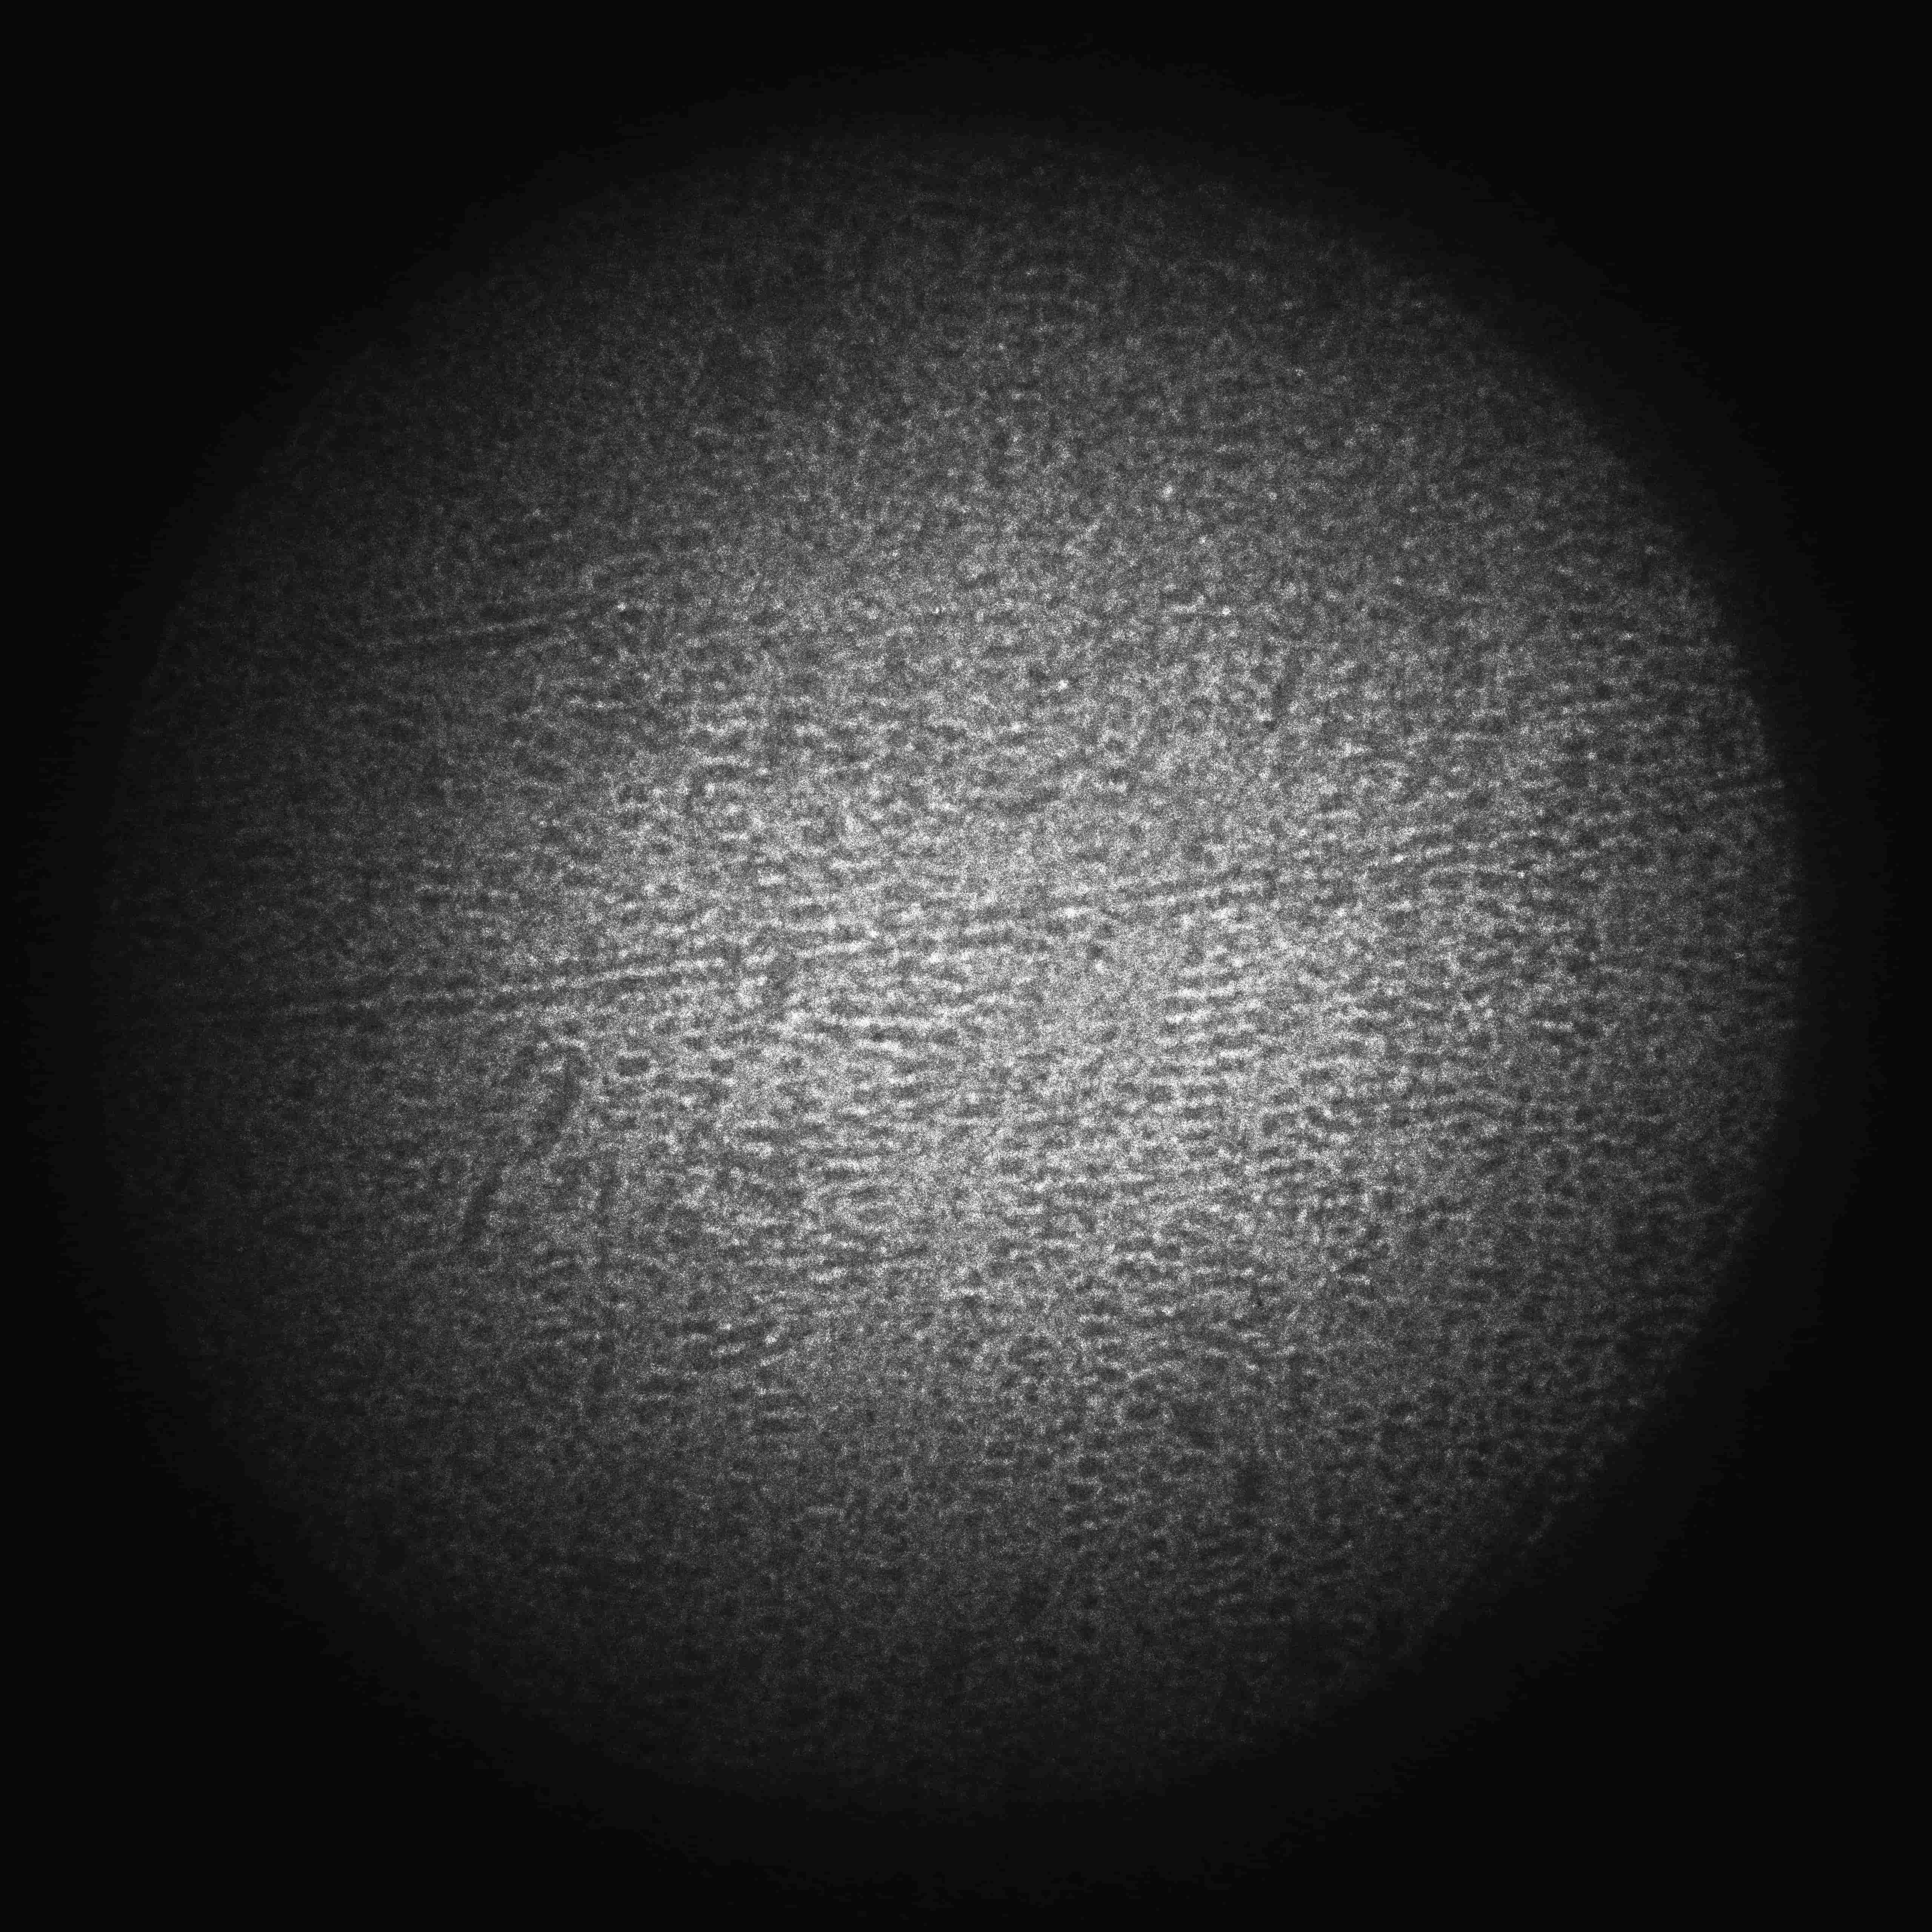
\includegraphics[height=0.3\textwidth]{fig/convection_photos/2mm_04.jpg}}
    \subfigure[$I=0.80$ A, $\Delta T=8.7\ ^\circ\text{C}$]{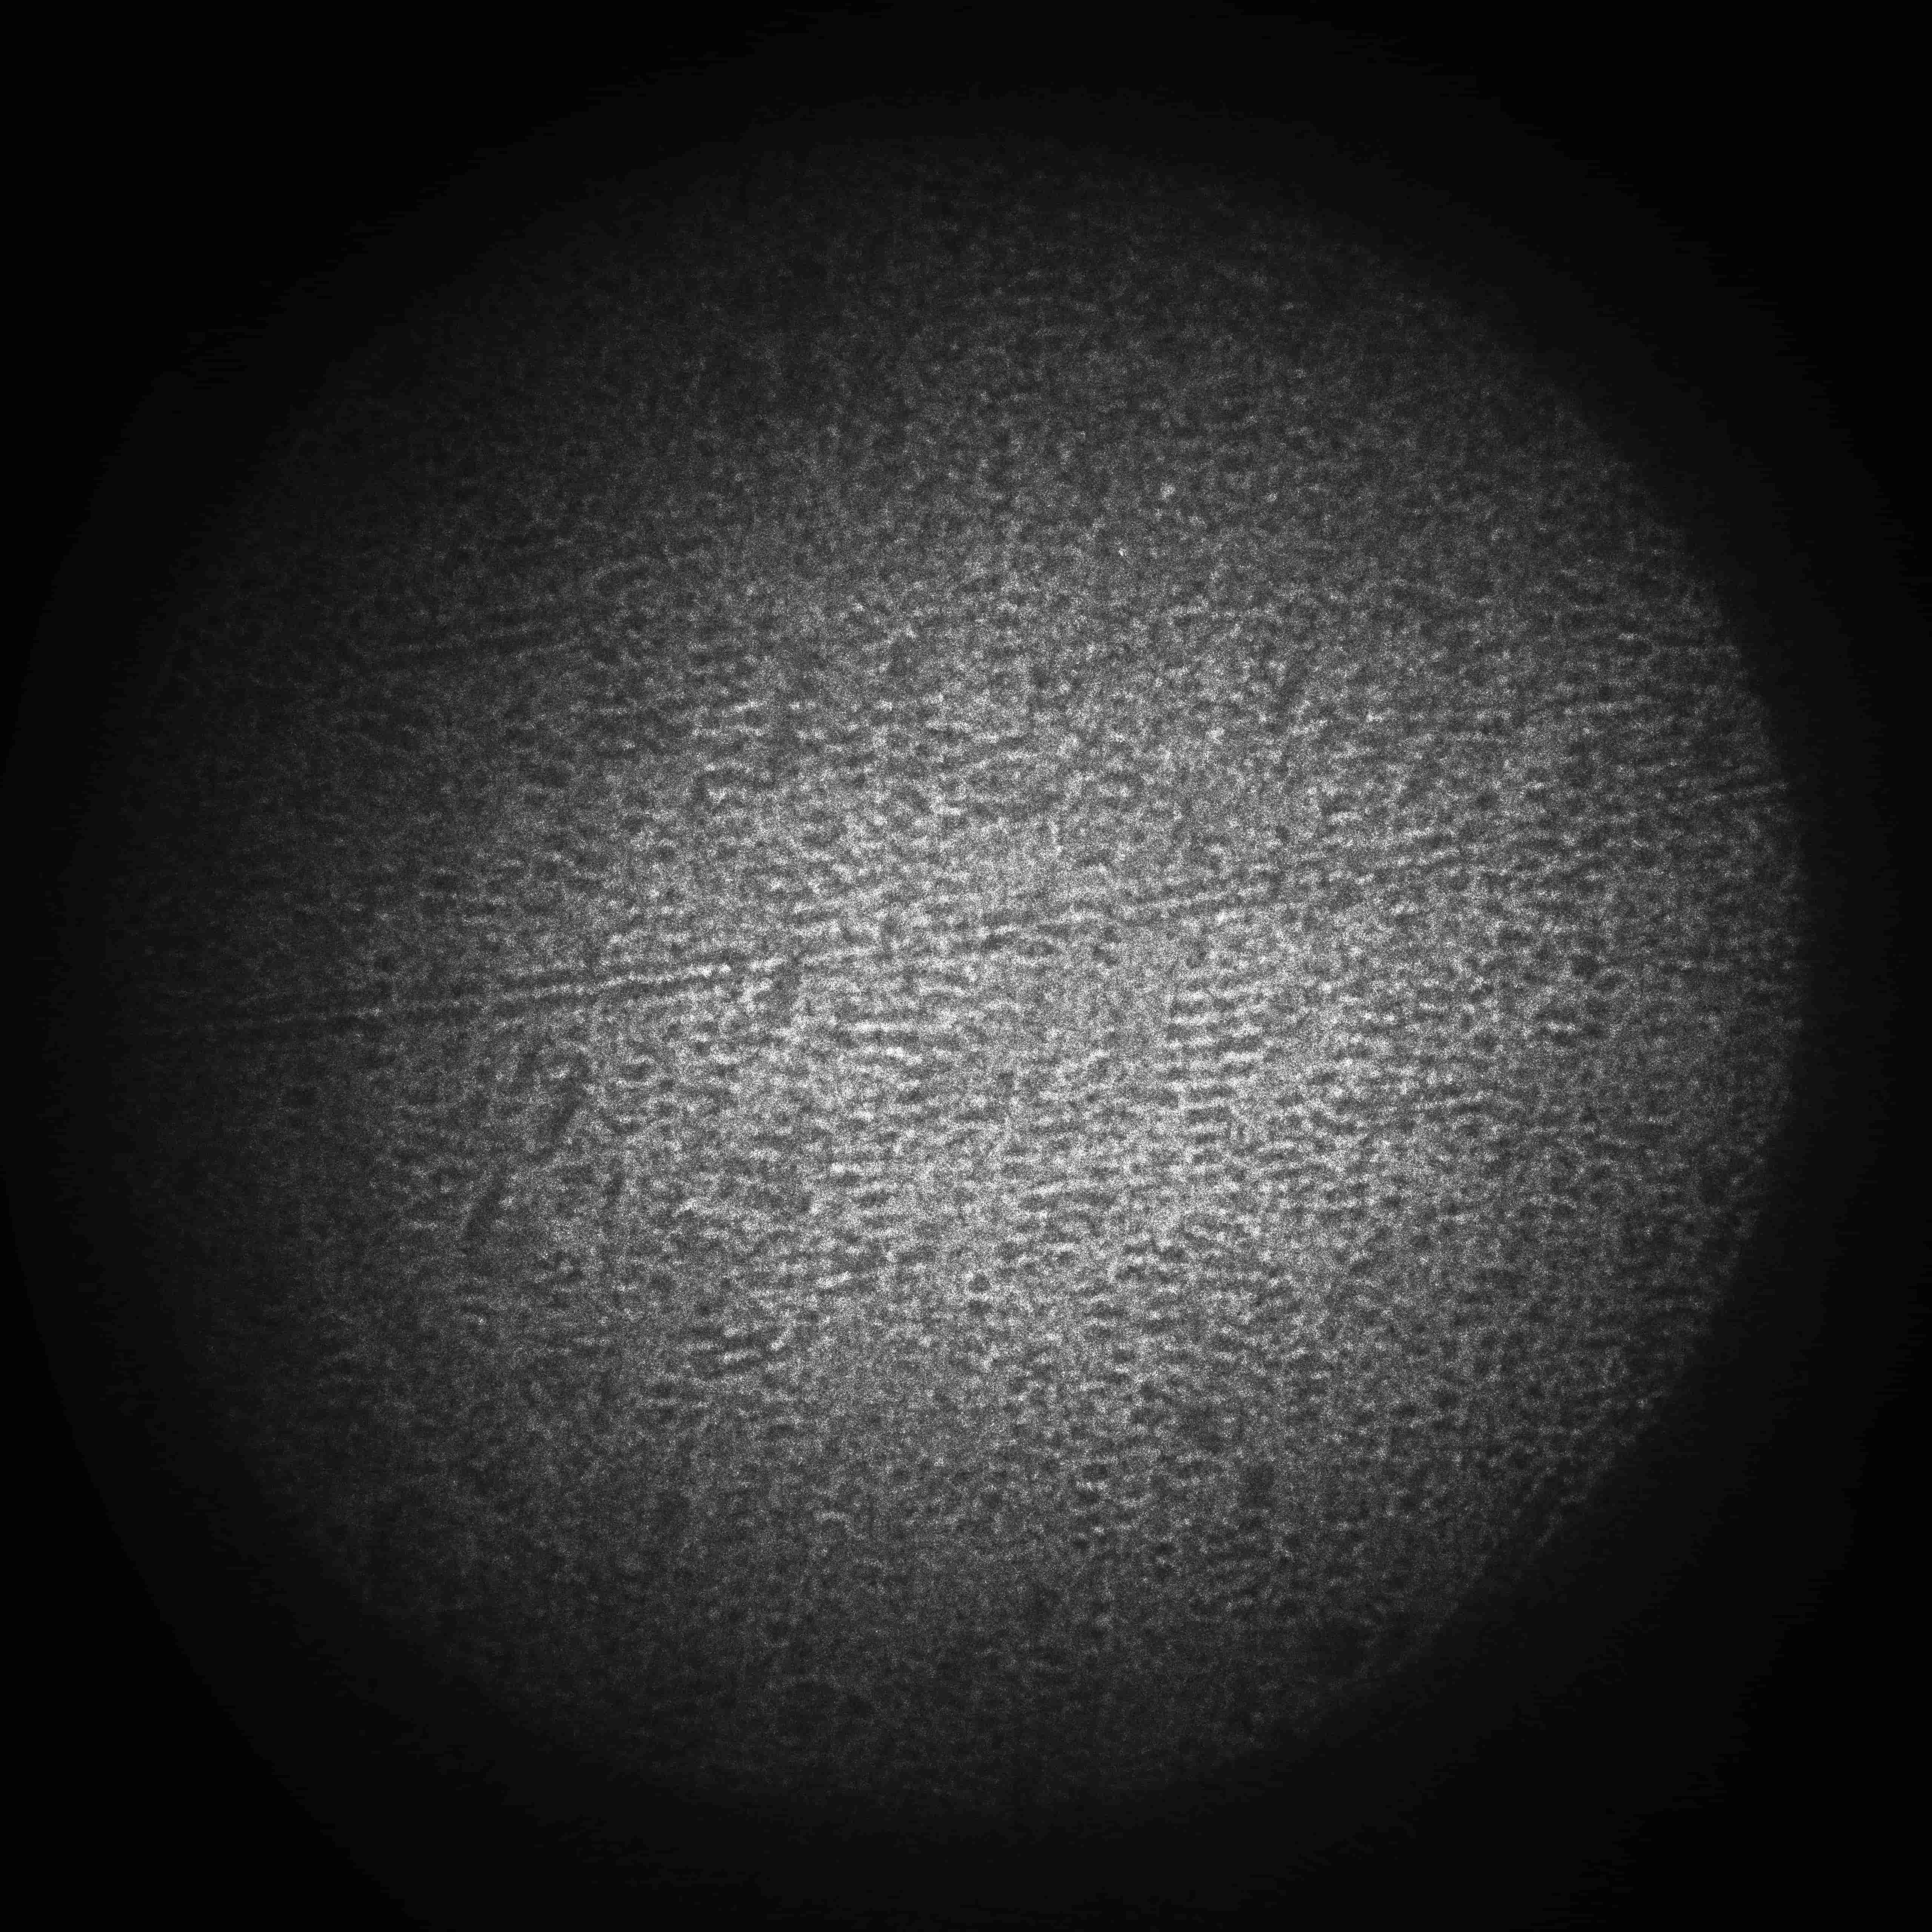
\includegraphics[height=0.3\textwidth]{fig/convection_photos/2mm_08.jpg}}
    \subfigure[$I=0.85$ A, $\Delta T=9.3\ ^\circ\text{C}$]{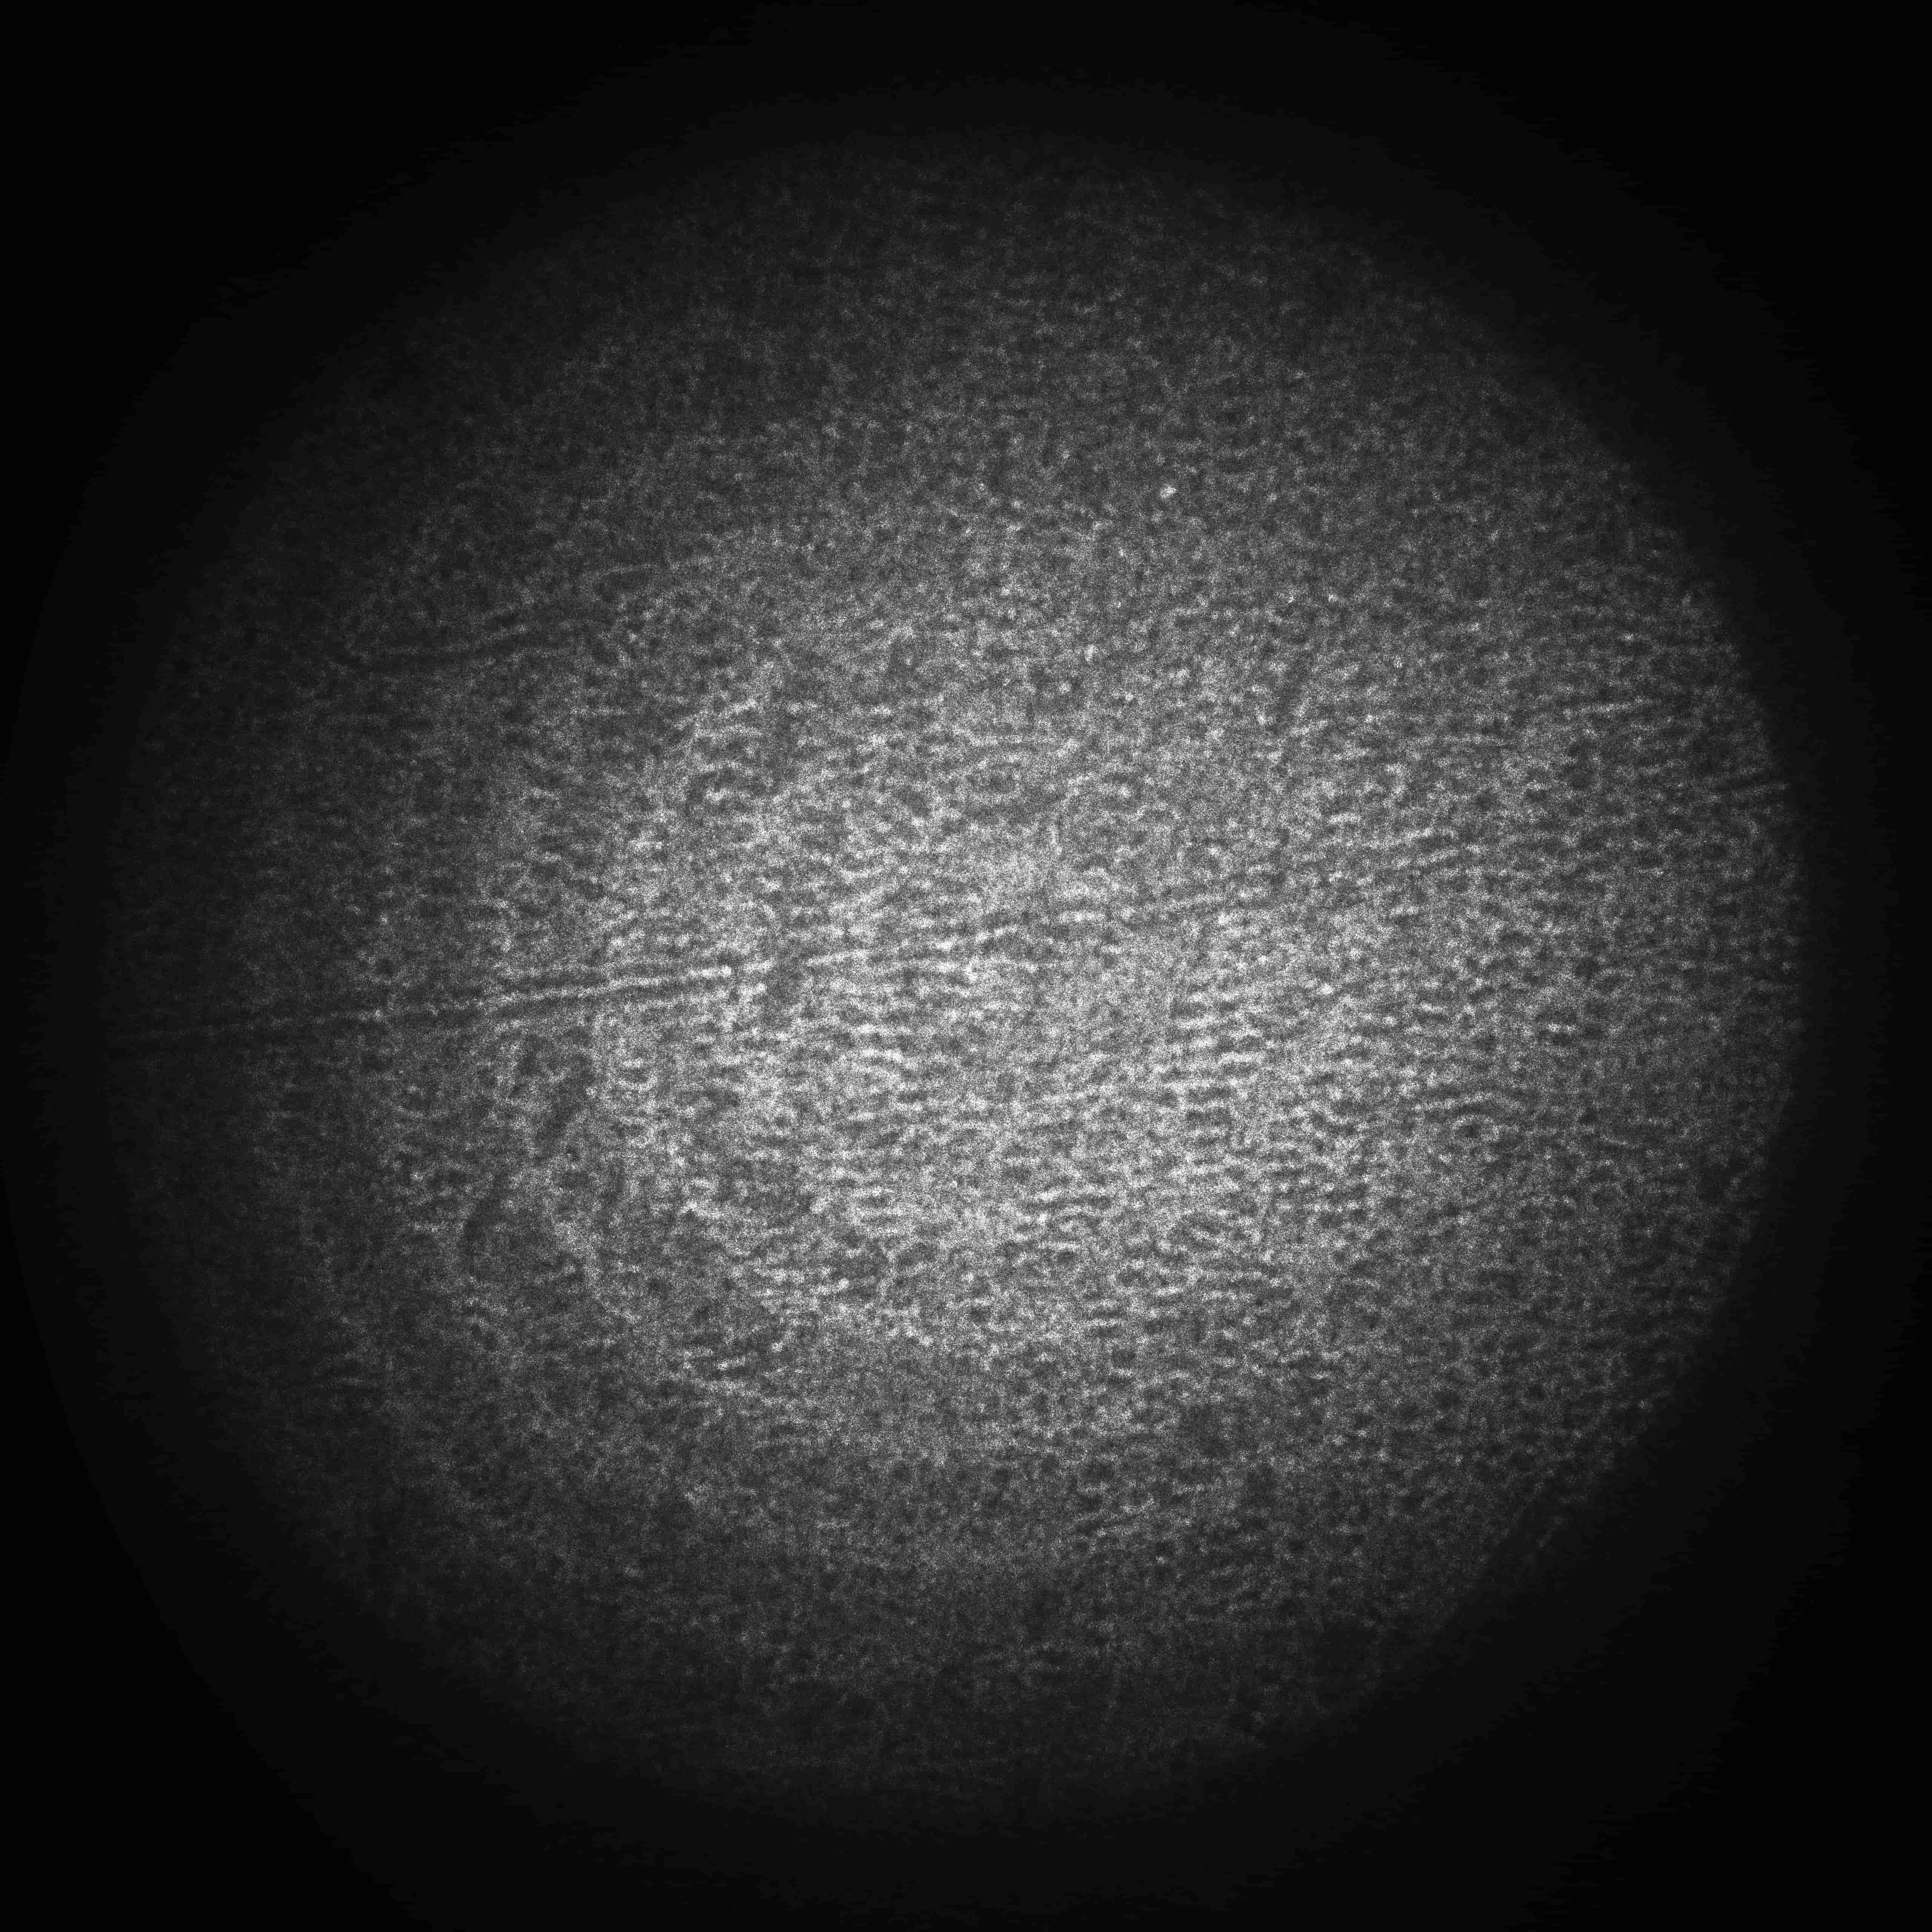
\includegraphics[height=0.3\textwidth]{fig/convection_photos/2mm_085.jpg}}
    \subfigure[$I=0.90$ A, $\Delta T=10.1\ ^\circ\text{C}$]{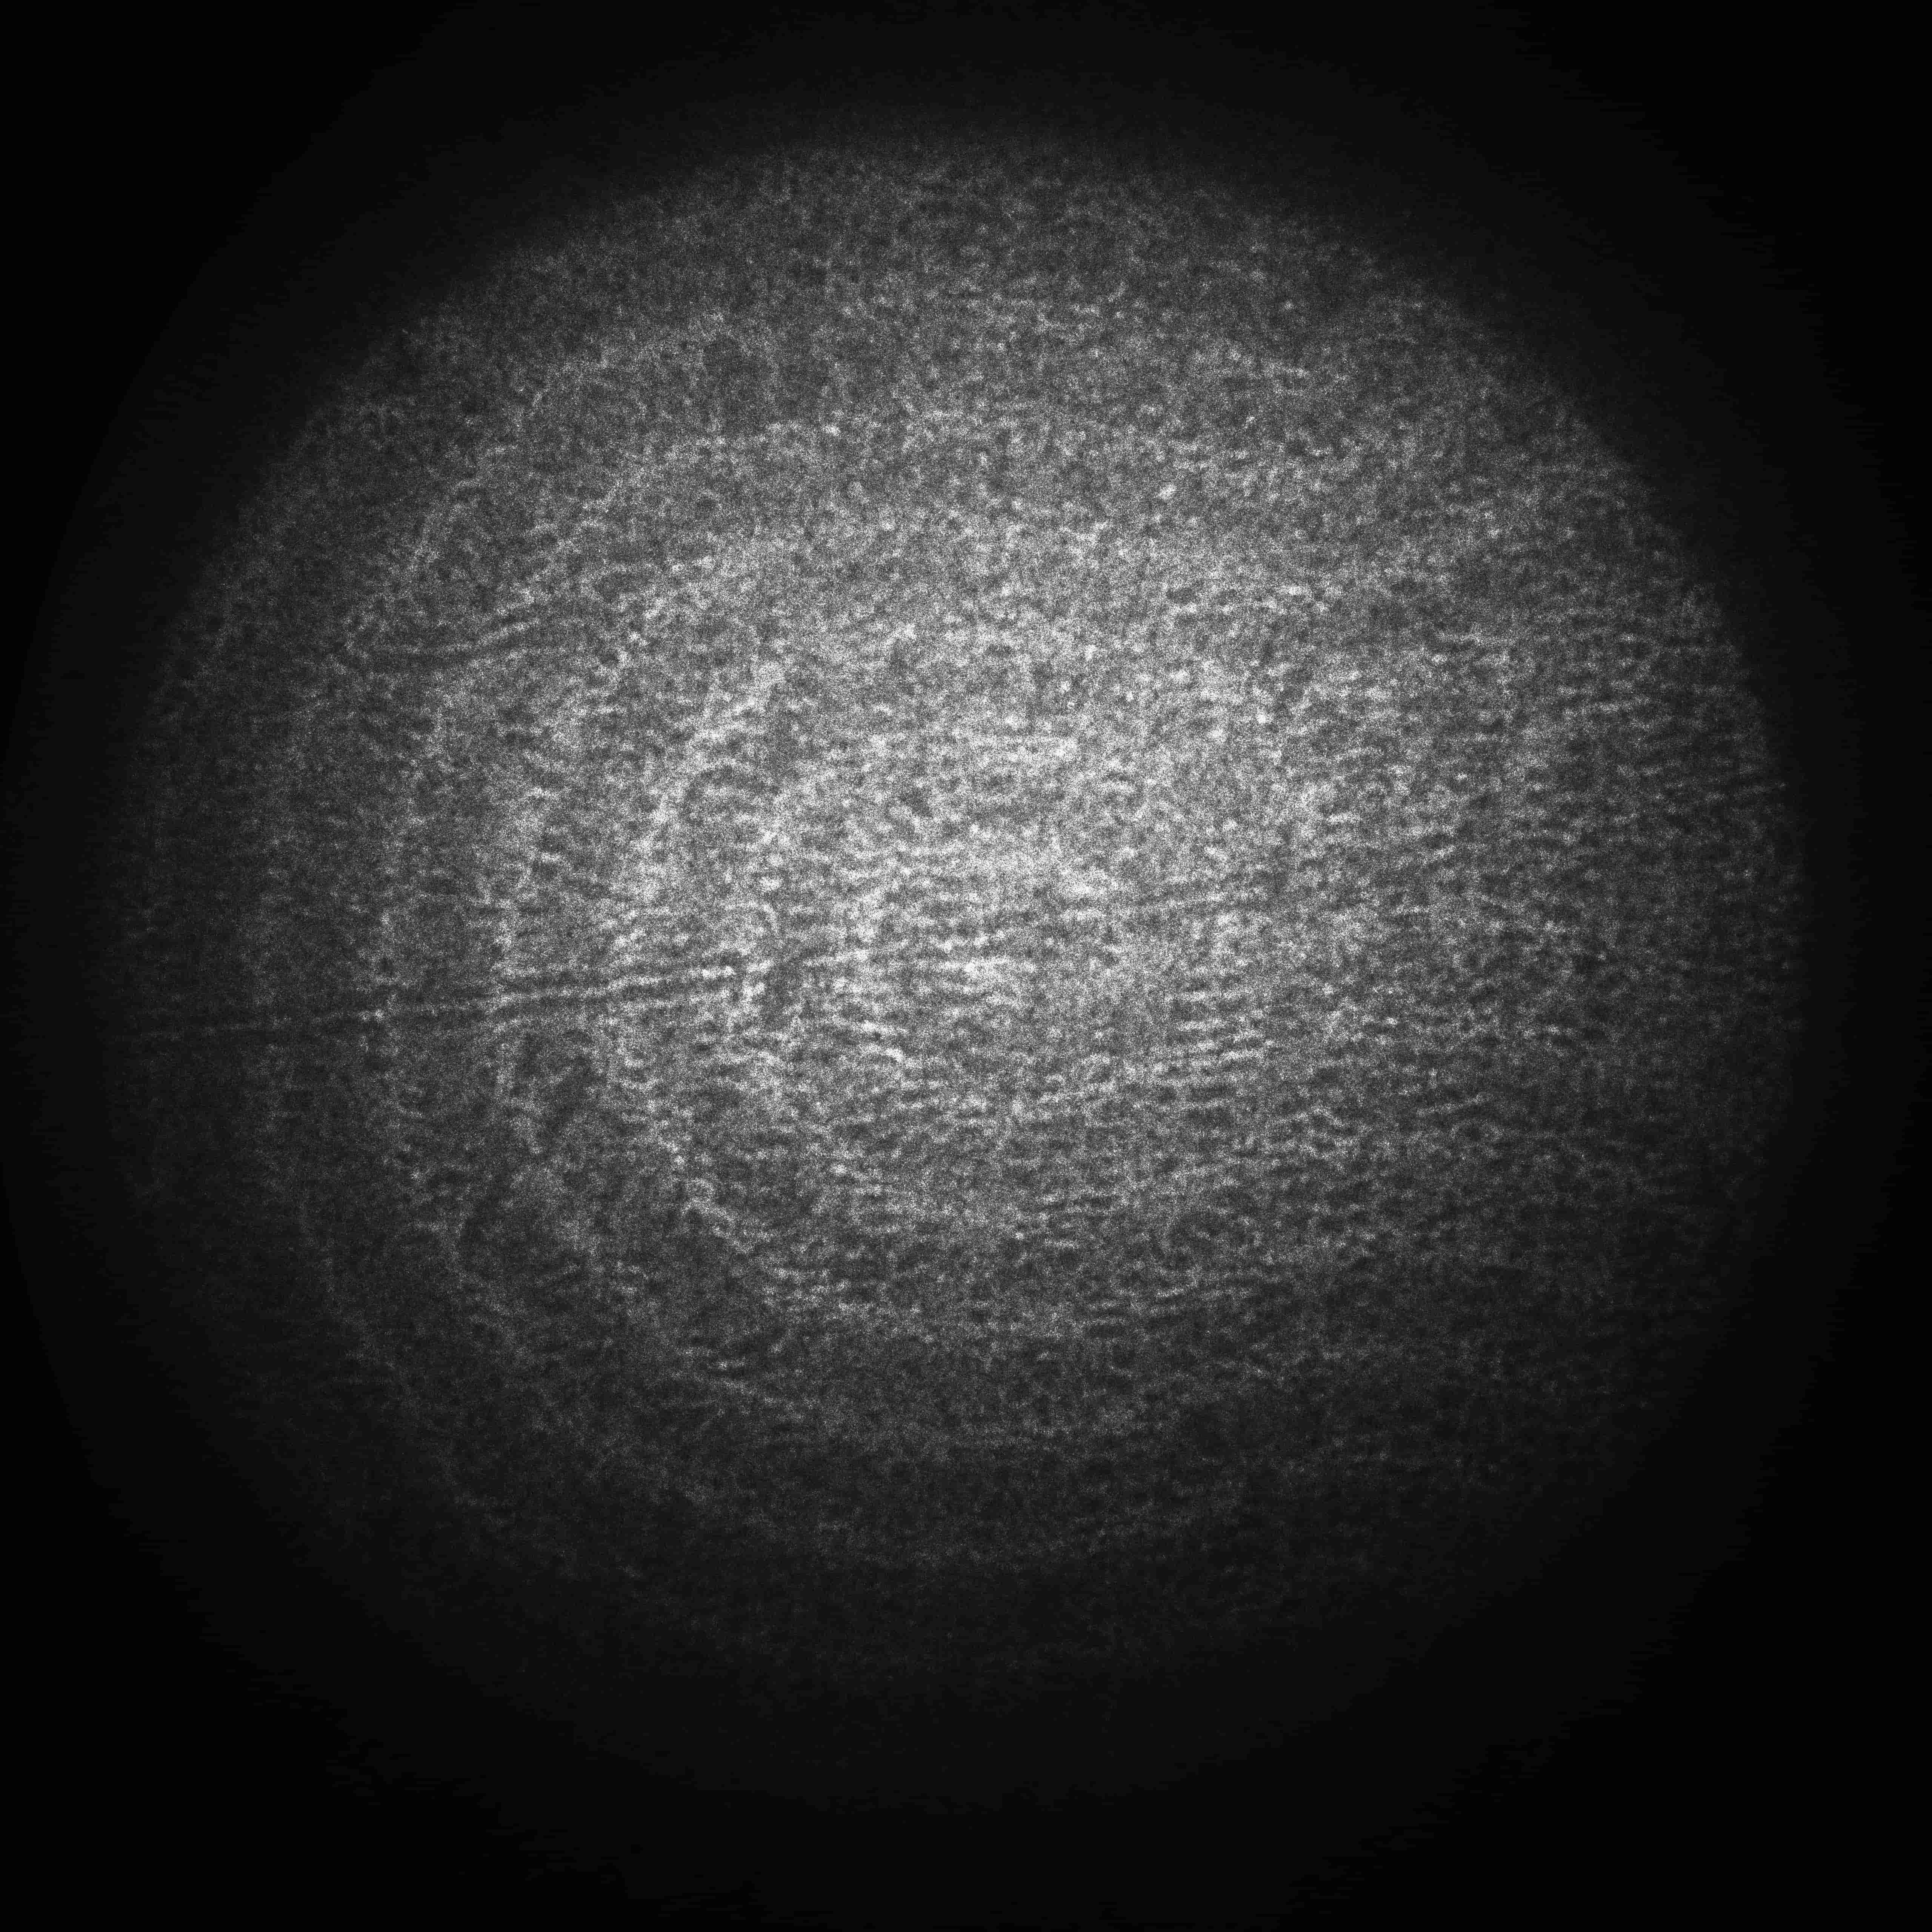
\includegraphics[height=0.3\textwidth]{fig/convection_photos/2mm_0901.jpg}}
    \subfigure[$I=1.00$ A, $\Delta T=11.4\ ^\circ\text{C}$]{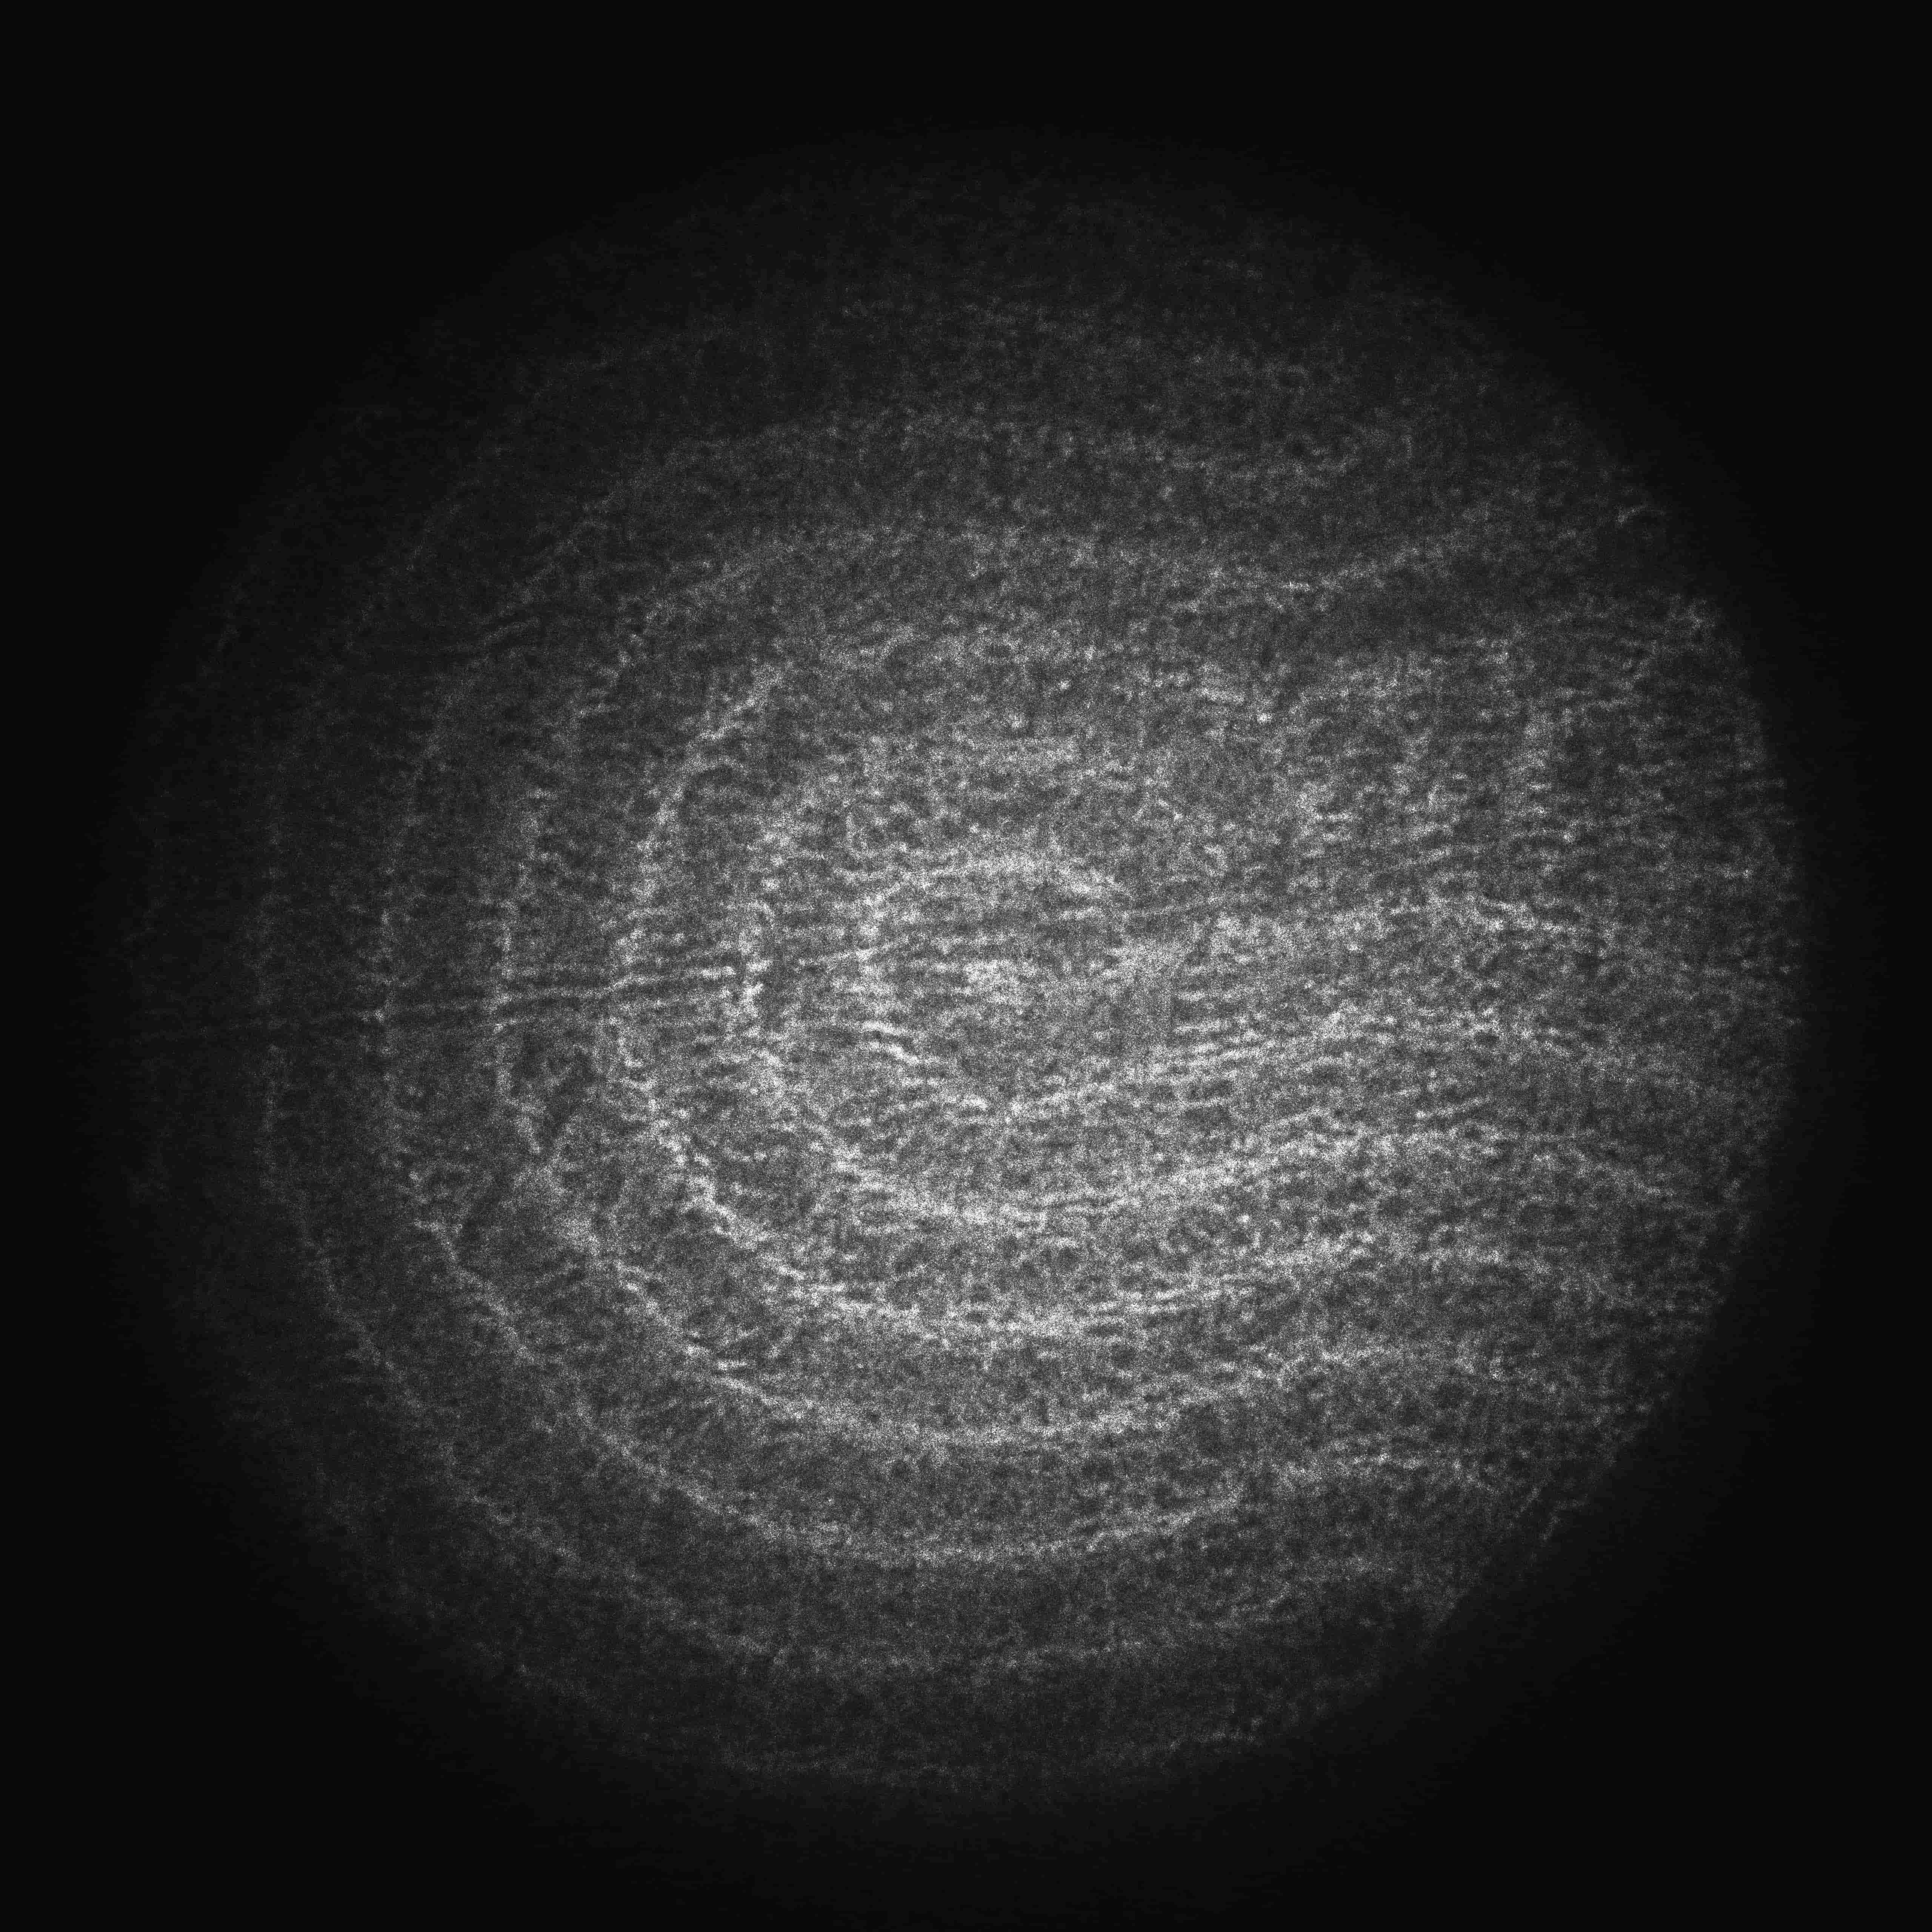
\includegraphics[height=0.3\textwidth]{fig/convection_photos/2mm_1003.jpg}}
    \subfigure[$I=1.20$ A, $\Delta T=14.3\ ^\circ\text{C}$]{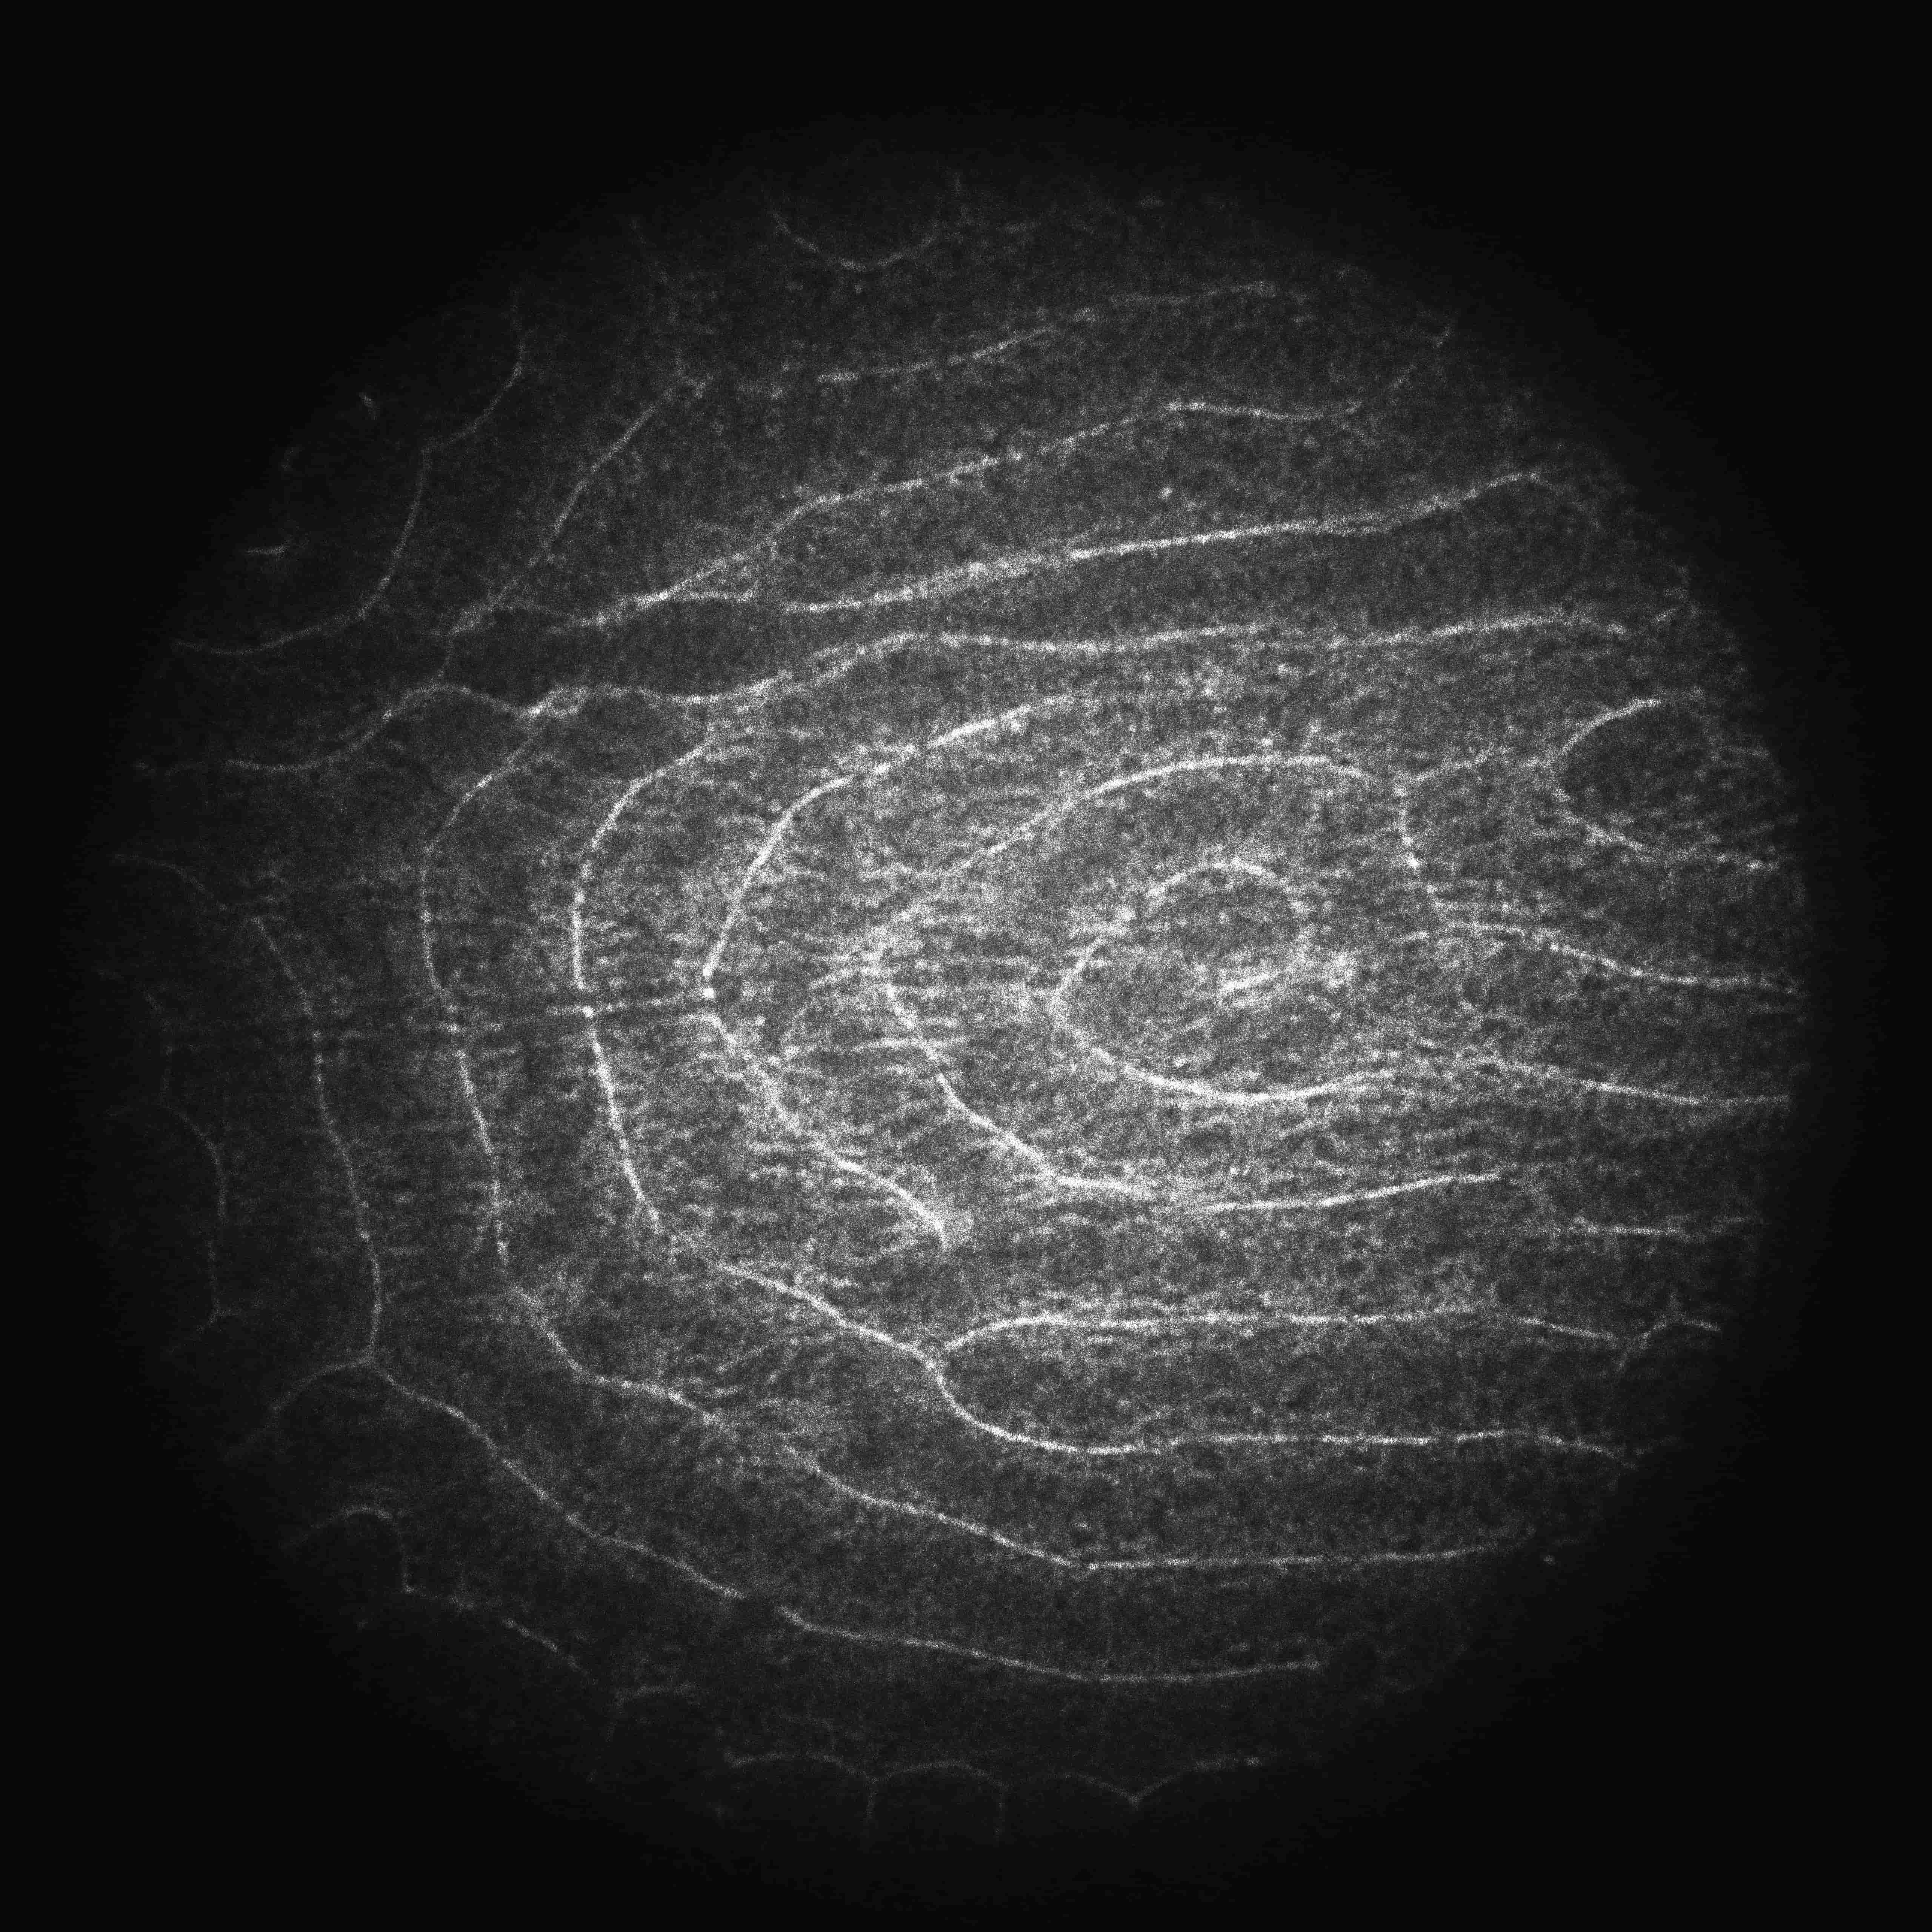
\includegraphics[height=0.3\textwidth]{fig/convection_photos/2mm_1193.jpg}}
    \caption{不同温度差下CCD拍摄得到的斑图。水层厚度$d=2$ mm。}
    \label{fig:convection_photos_2mm}
\end{figure}

首先我们观察水层厚度为2 mm的结果(\autoref{fig:convection_photos_2mm})。我们可以清楚的看到,随着温度差的增加,斑图从无到有的演化:在\autoref{fig:convection_photos_2mm}(b) 中,我们已经可以隐约看到斑图的出现,因此我们得到临界点的温度差约为$\Delta T=8.7\ ^\circ\text{C}$。随后斑图越来越明显,直到温度差的进一步加大导致原来的斑图发生了结构上的改变(\autoref{fig:convection_photos_2mm}(f))。

值得说明的是,由于我们实验中选取的系统具有圆对称性,我们期待斑图也具有圆对称性。但是在实验过程中,我们的斑图变为螺旋形。这是因为系统的演化会同时受到初始条件和边界条件的限制。在实验中,我们控制初始条件的方式是:在实验前通过静置对流水层一段时间,使其进入内部没有任何流动的稳定状态($\bm{v}=0$)。但是在本次实验中,我们静置水层的时间仍然不够长(我们静置了约40 min,但实际上可能需要1 h),导致初始水层中有不对称的流速场分布,这就使得当系统从无序状态向有序状态演化的时候,没有办法保持宏观的圆对称性。

另外,我们观察到随着温差的增大,对流元胞的尺度会有所增大,但是当温差大到一定程度的时候,增大的对流元胞也难以满足热量传输的需求,斑图的构型发生变化。从\autoref{fig:convection_photos_2mm}(e) 到\autoref{fig:convection_photos_2mm}(f) 可以看到,斑图原来的构型被破坏,并且出现了很多对流的奇点(多条白色条纹交汇的地方)。特别是在圆边缘处,出现了很多角向分布的对流元胞。
\begin{figure}
    \centering
    \subfigure[$I=0.20$ A, $\Delta T=1.3\ ^\circ\text{C}$]{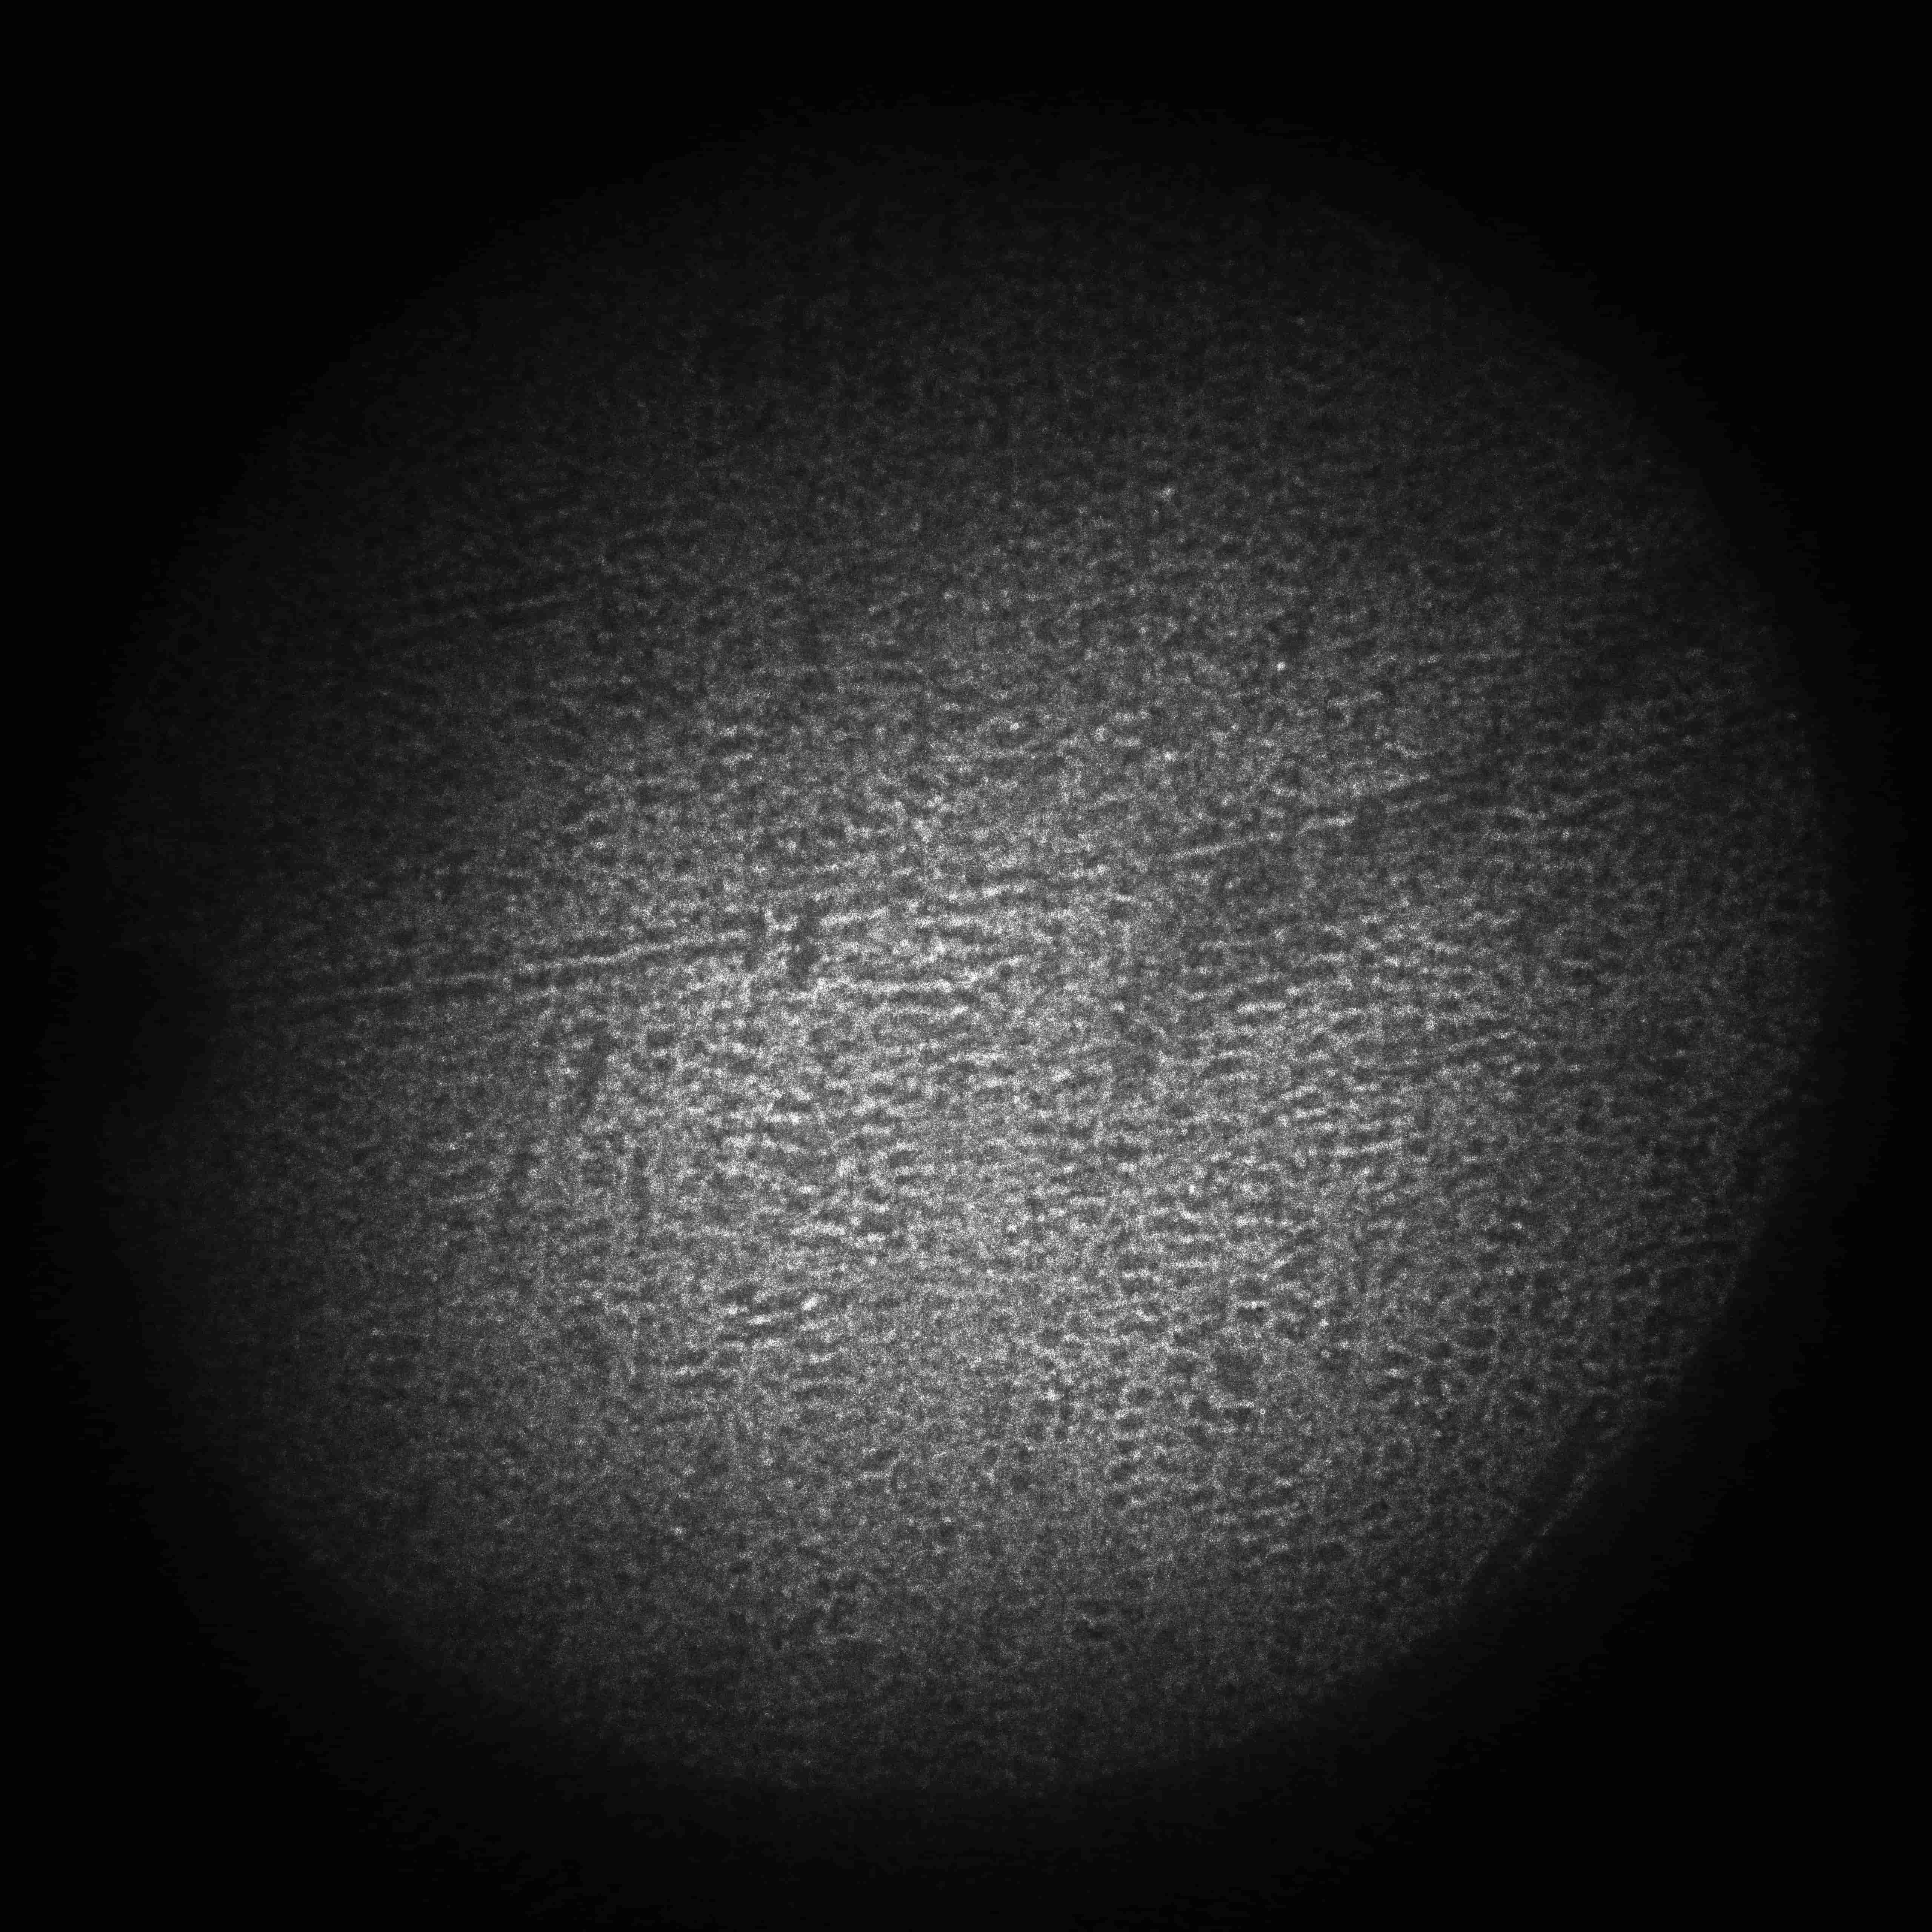
\includegraphics[height=0.3\textwidth]{fig/convection_photos/4mm_0202.jpg}}
    \subfigure[$I=0.60$ A, $\Delta T=4.8\ ^\circ\text{C}$]{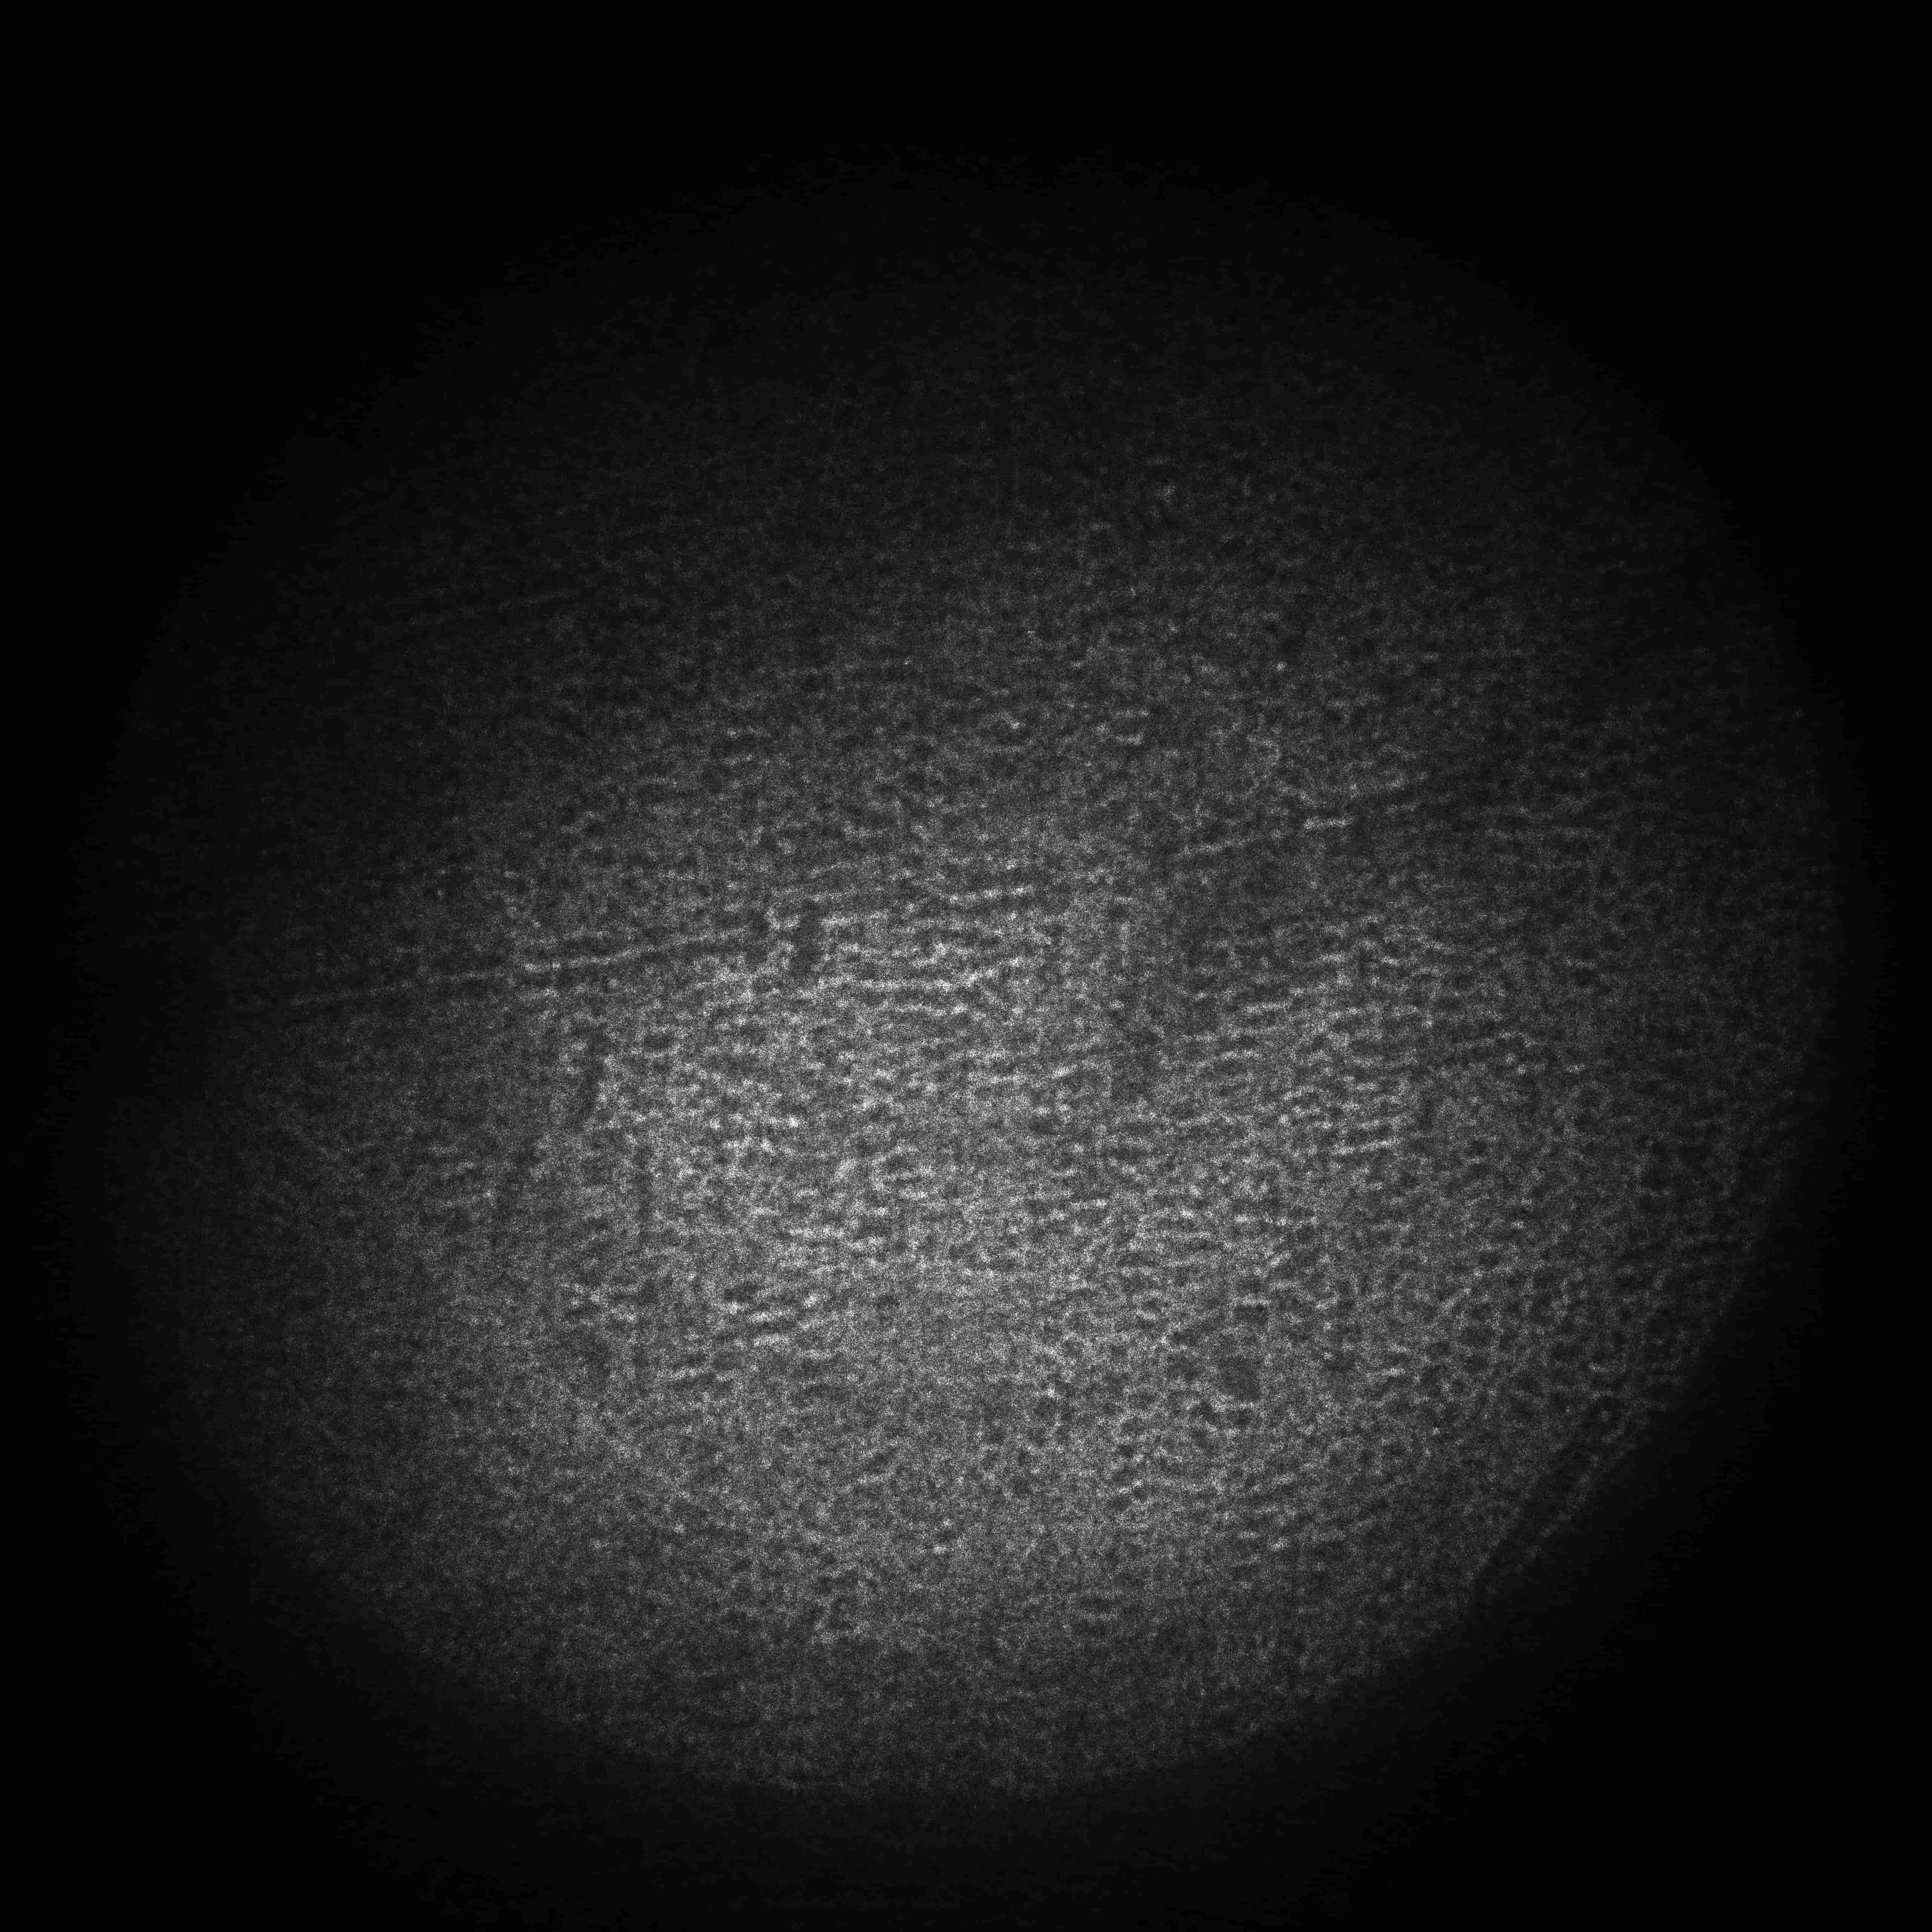
\includegraphics[height=0.3\textwidth]{fig/convection_photos/4mm_0599.jpg}}
    \subfigure[$I=0.90$ A, $\Delta T=9.3\ ^\circ\text{C}$]{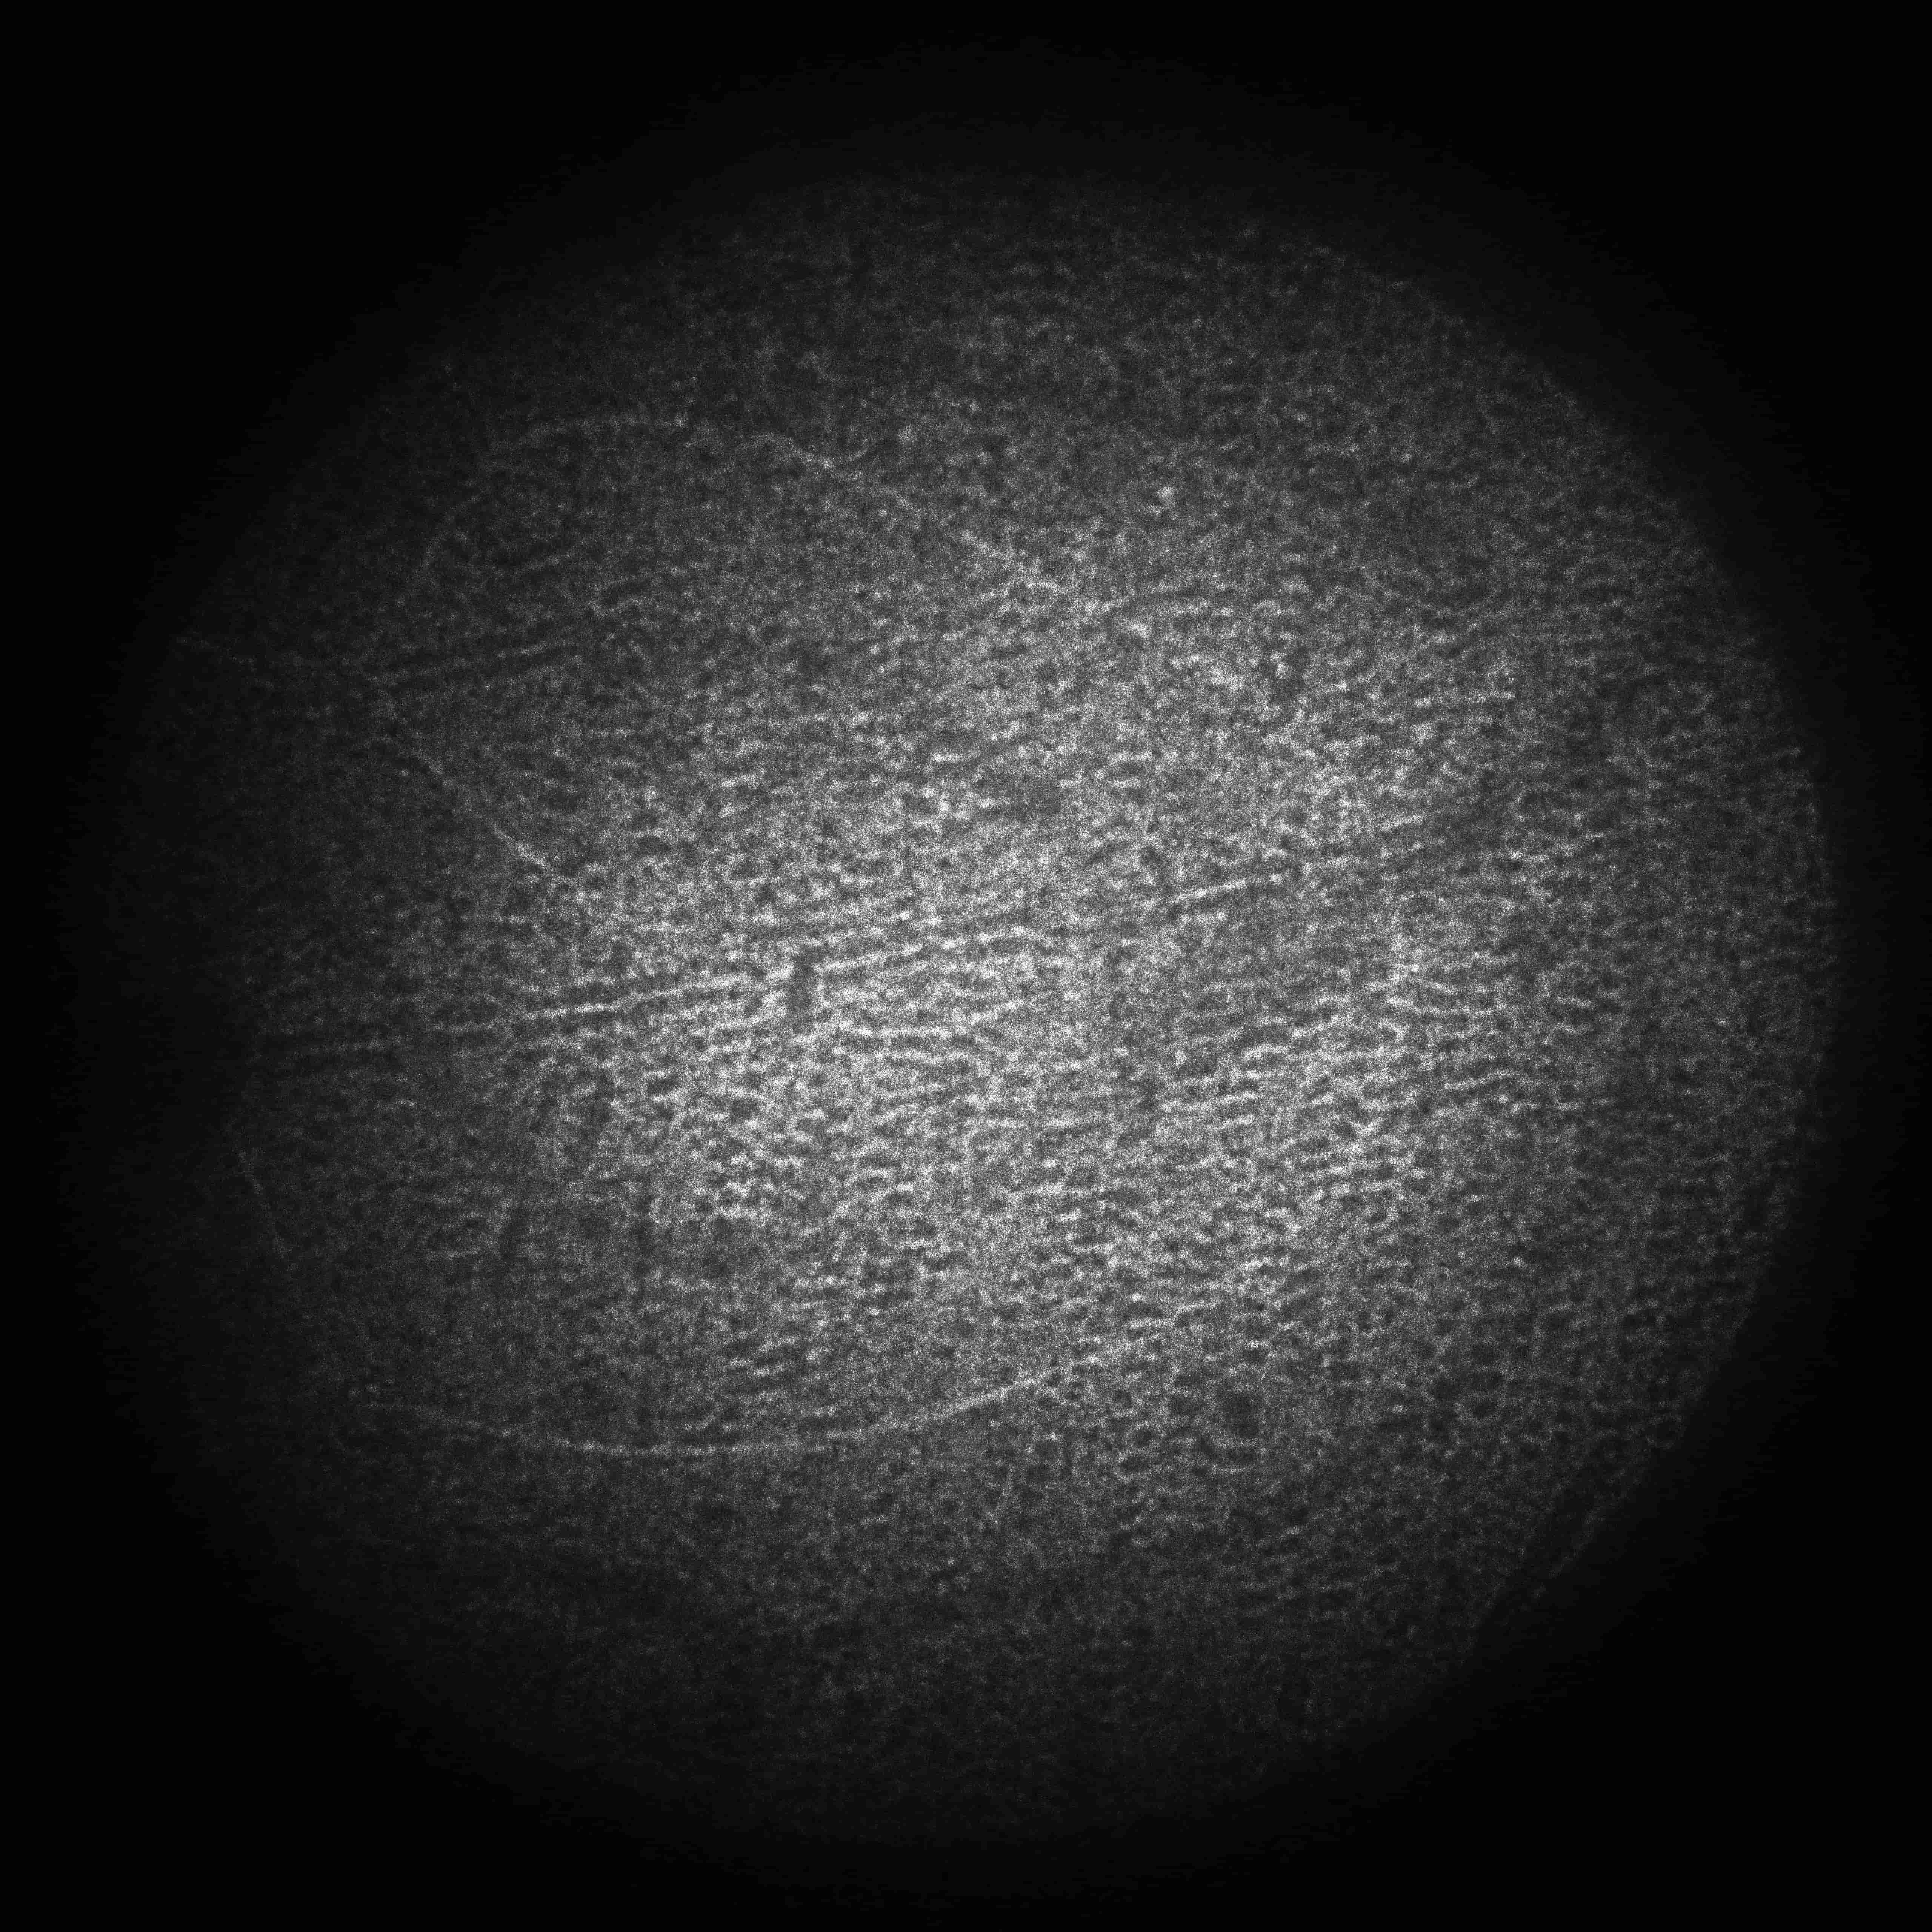
\includegraphics[height=0.3\textwidth]{fig/convection_photos/4mm_0899.jpg}}
    \subfigure[$I=1.20$ A, $\Delta T=14.6\ ^\circ\text{C}$]{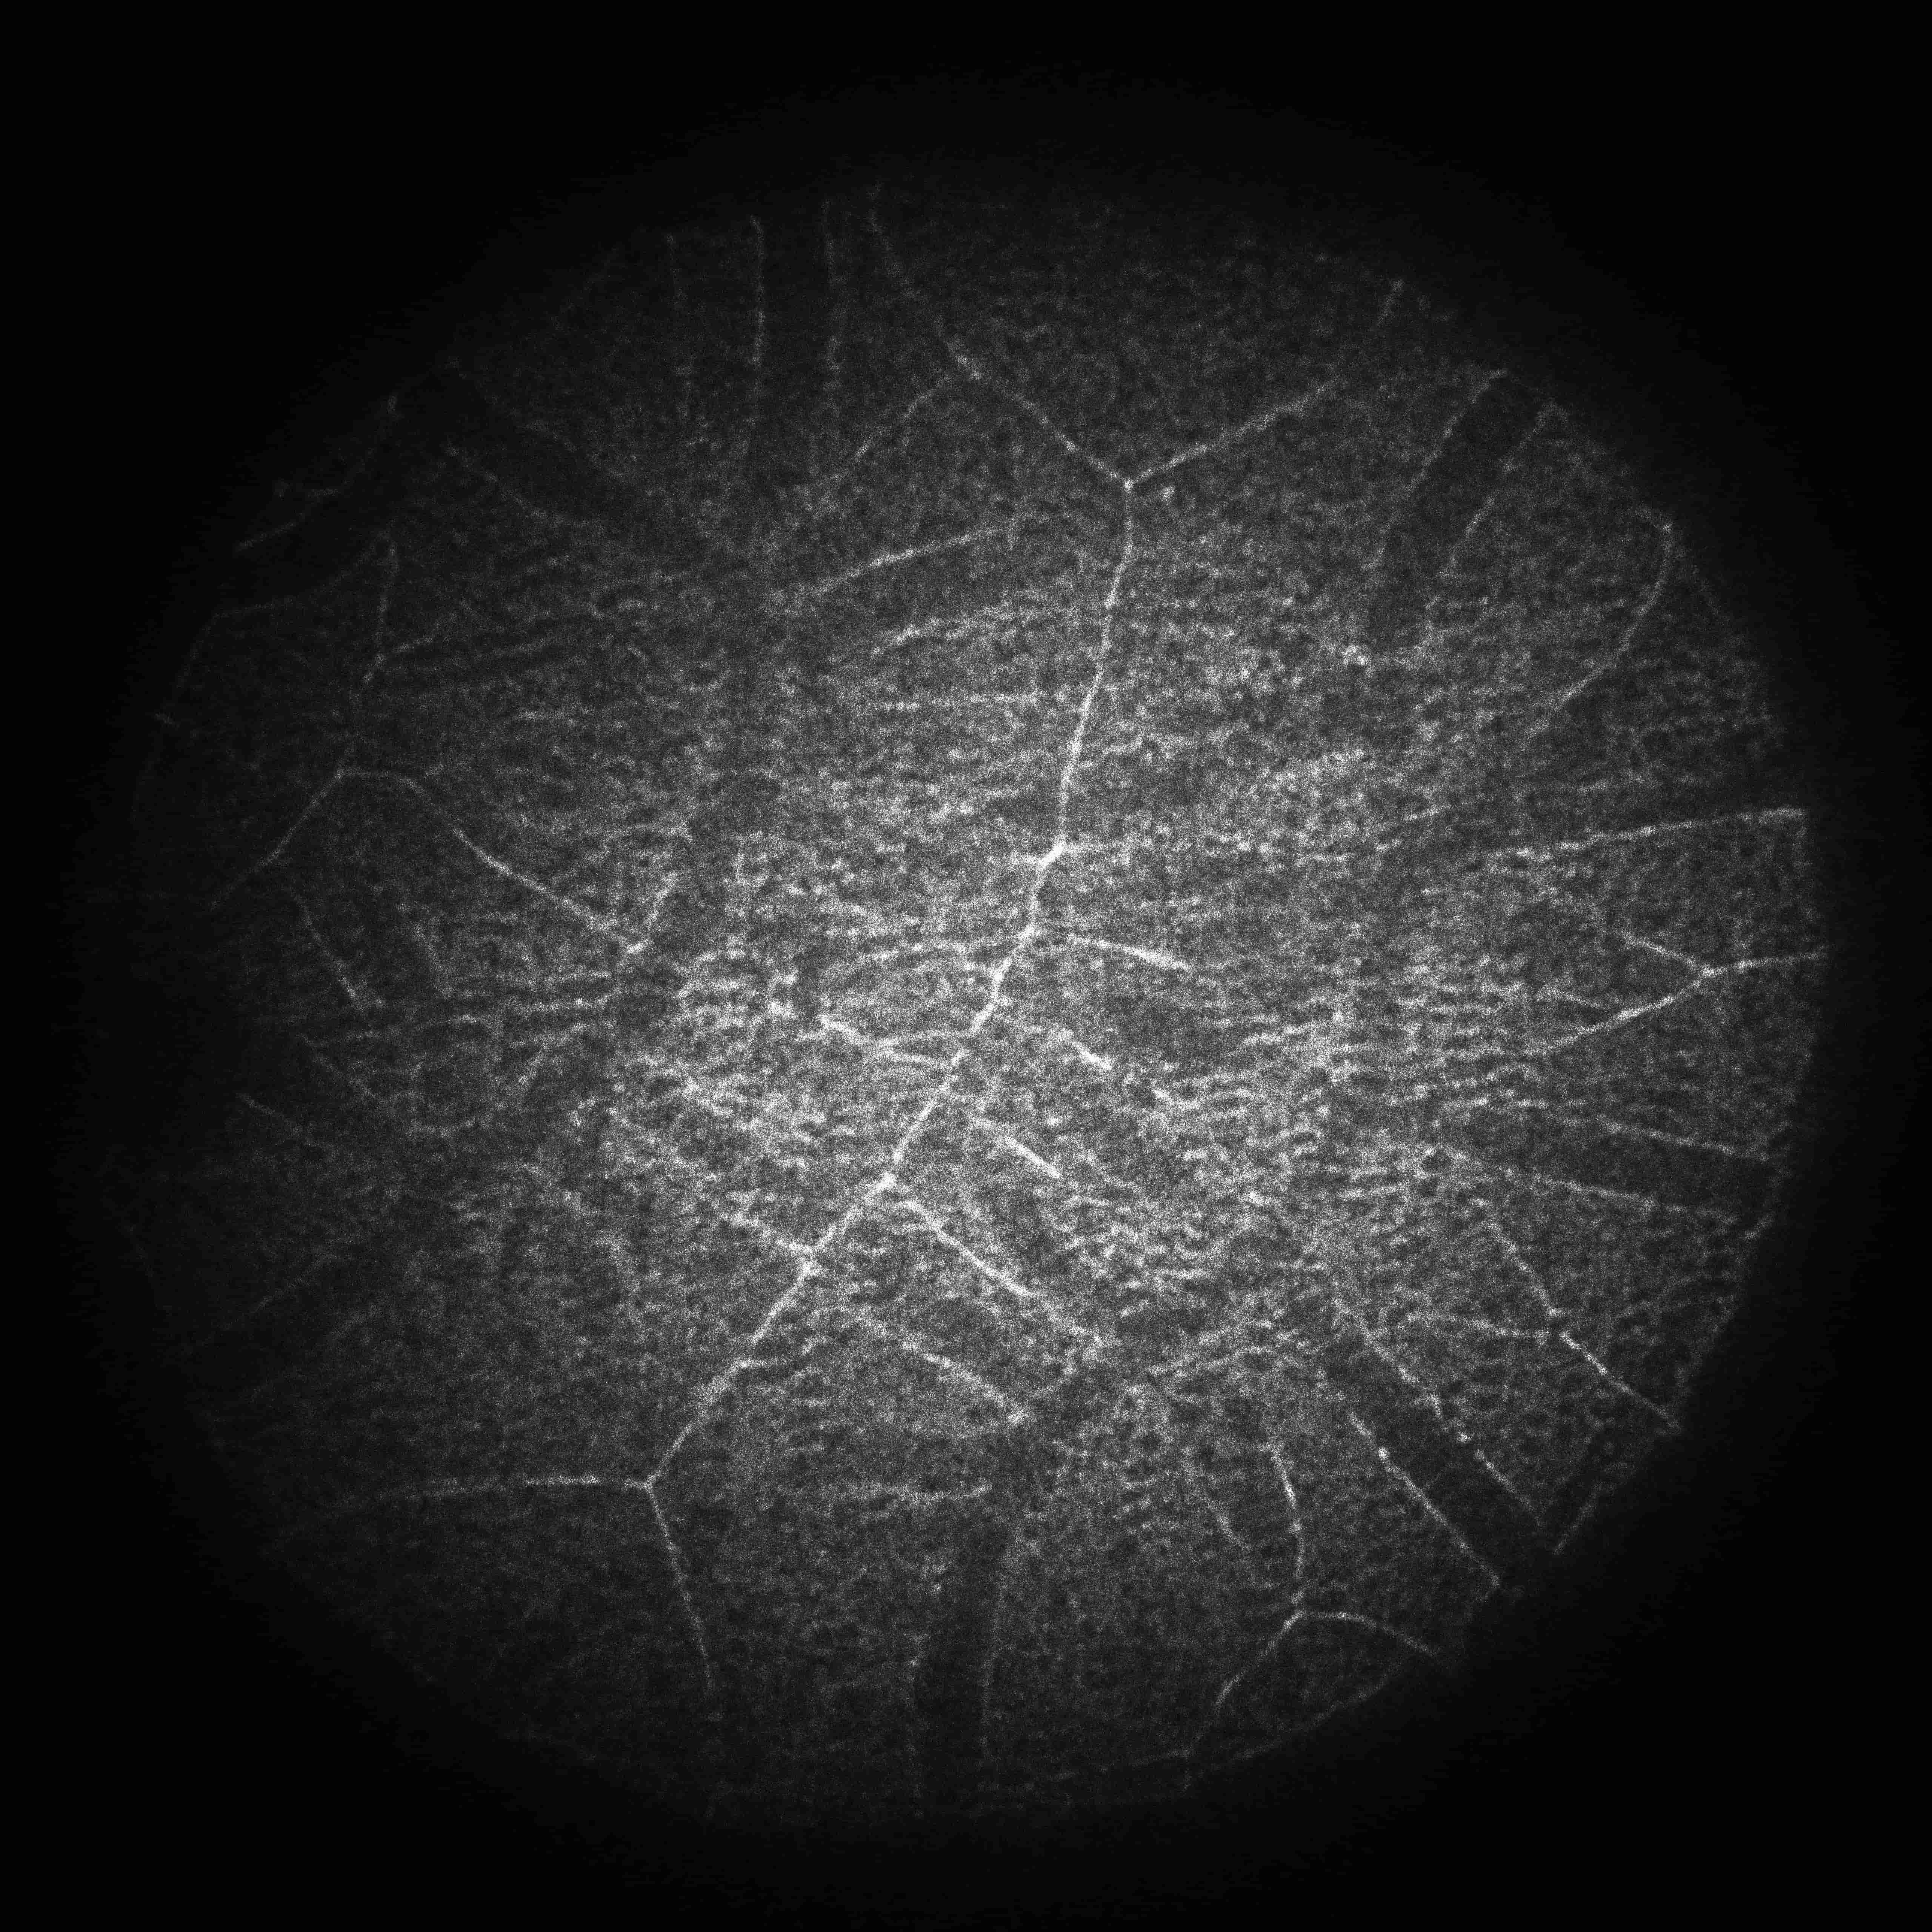
\includegraphics[height=0.3\textwidth]{fig/convection_photos/4mm_1195.jpg}}
    \subfigure[$I=1.50$ A, $\Delta T=21.4\ ^\circ\text{C}$]{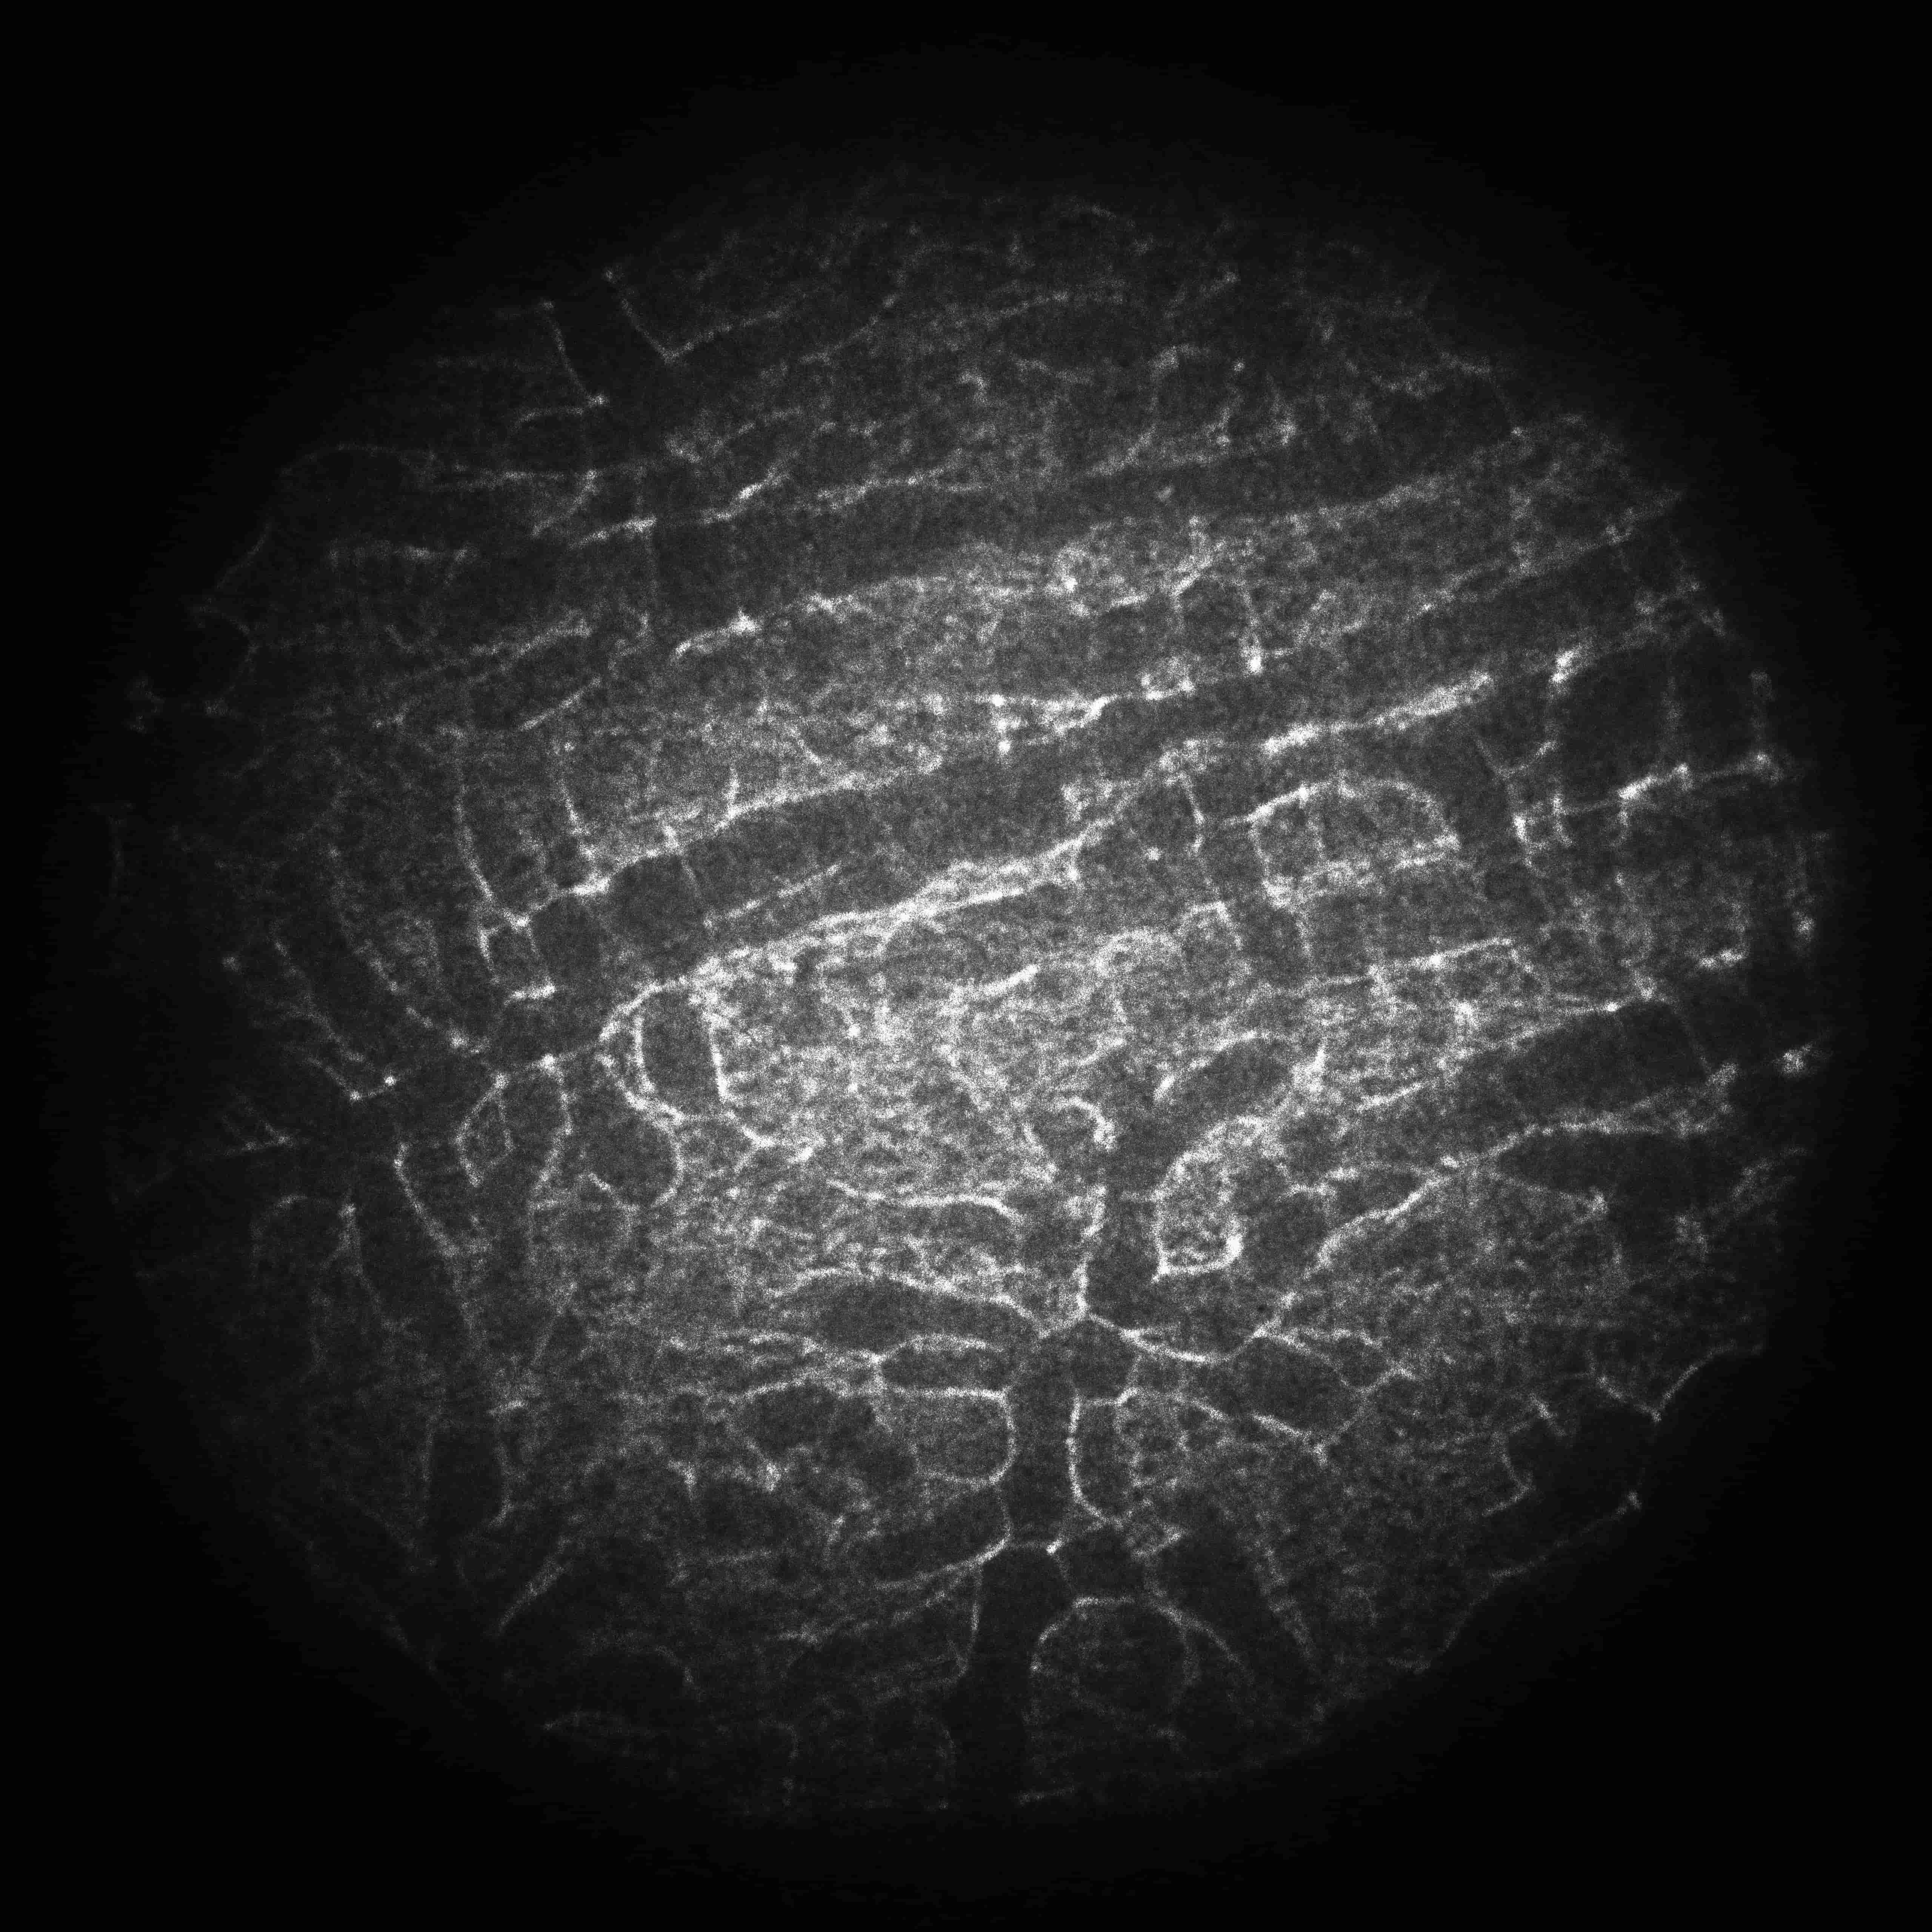
\includegraphics[height=0.3\textwidth]{fig/convection_photos/4mm_1496.jpg}}
    \subfigure[$I=1.80$ A, $\Delta T=28.2\ ^\circ\text{C}$]{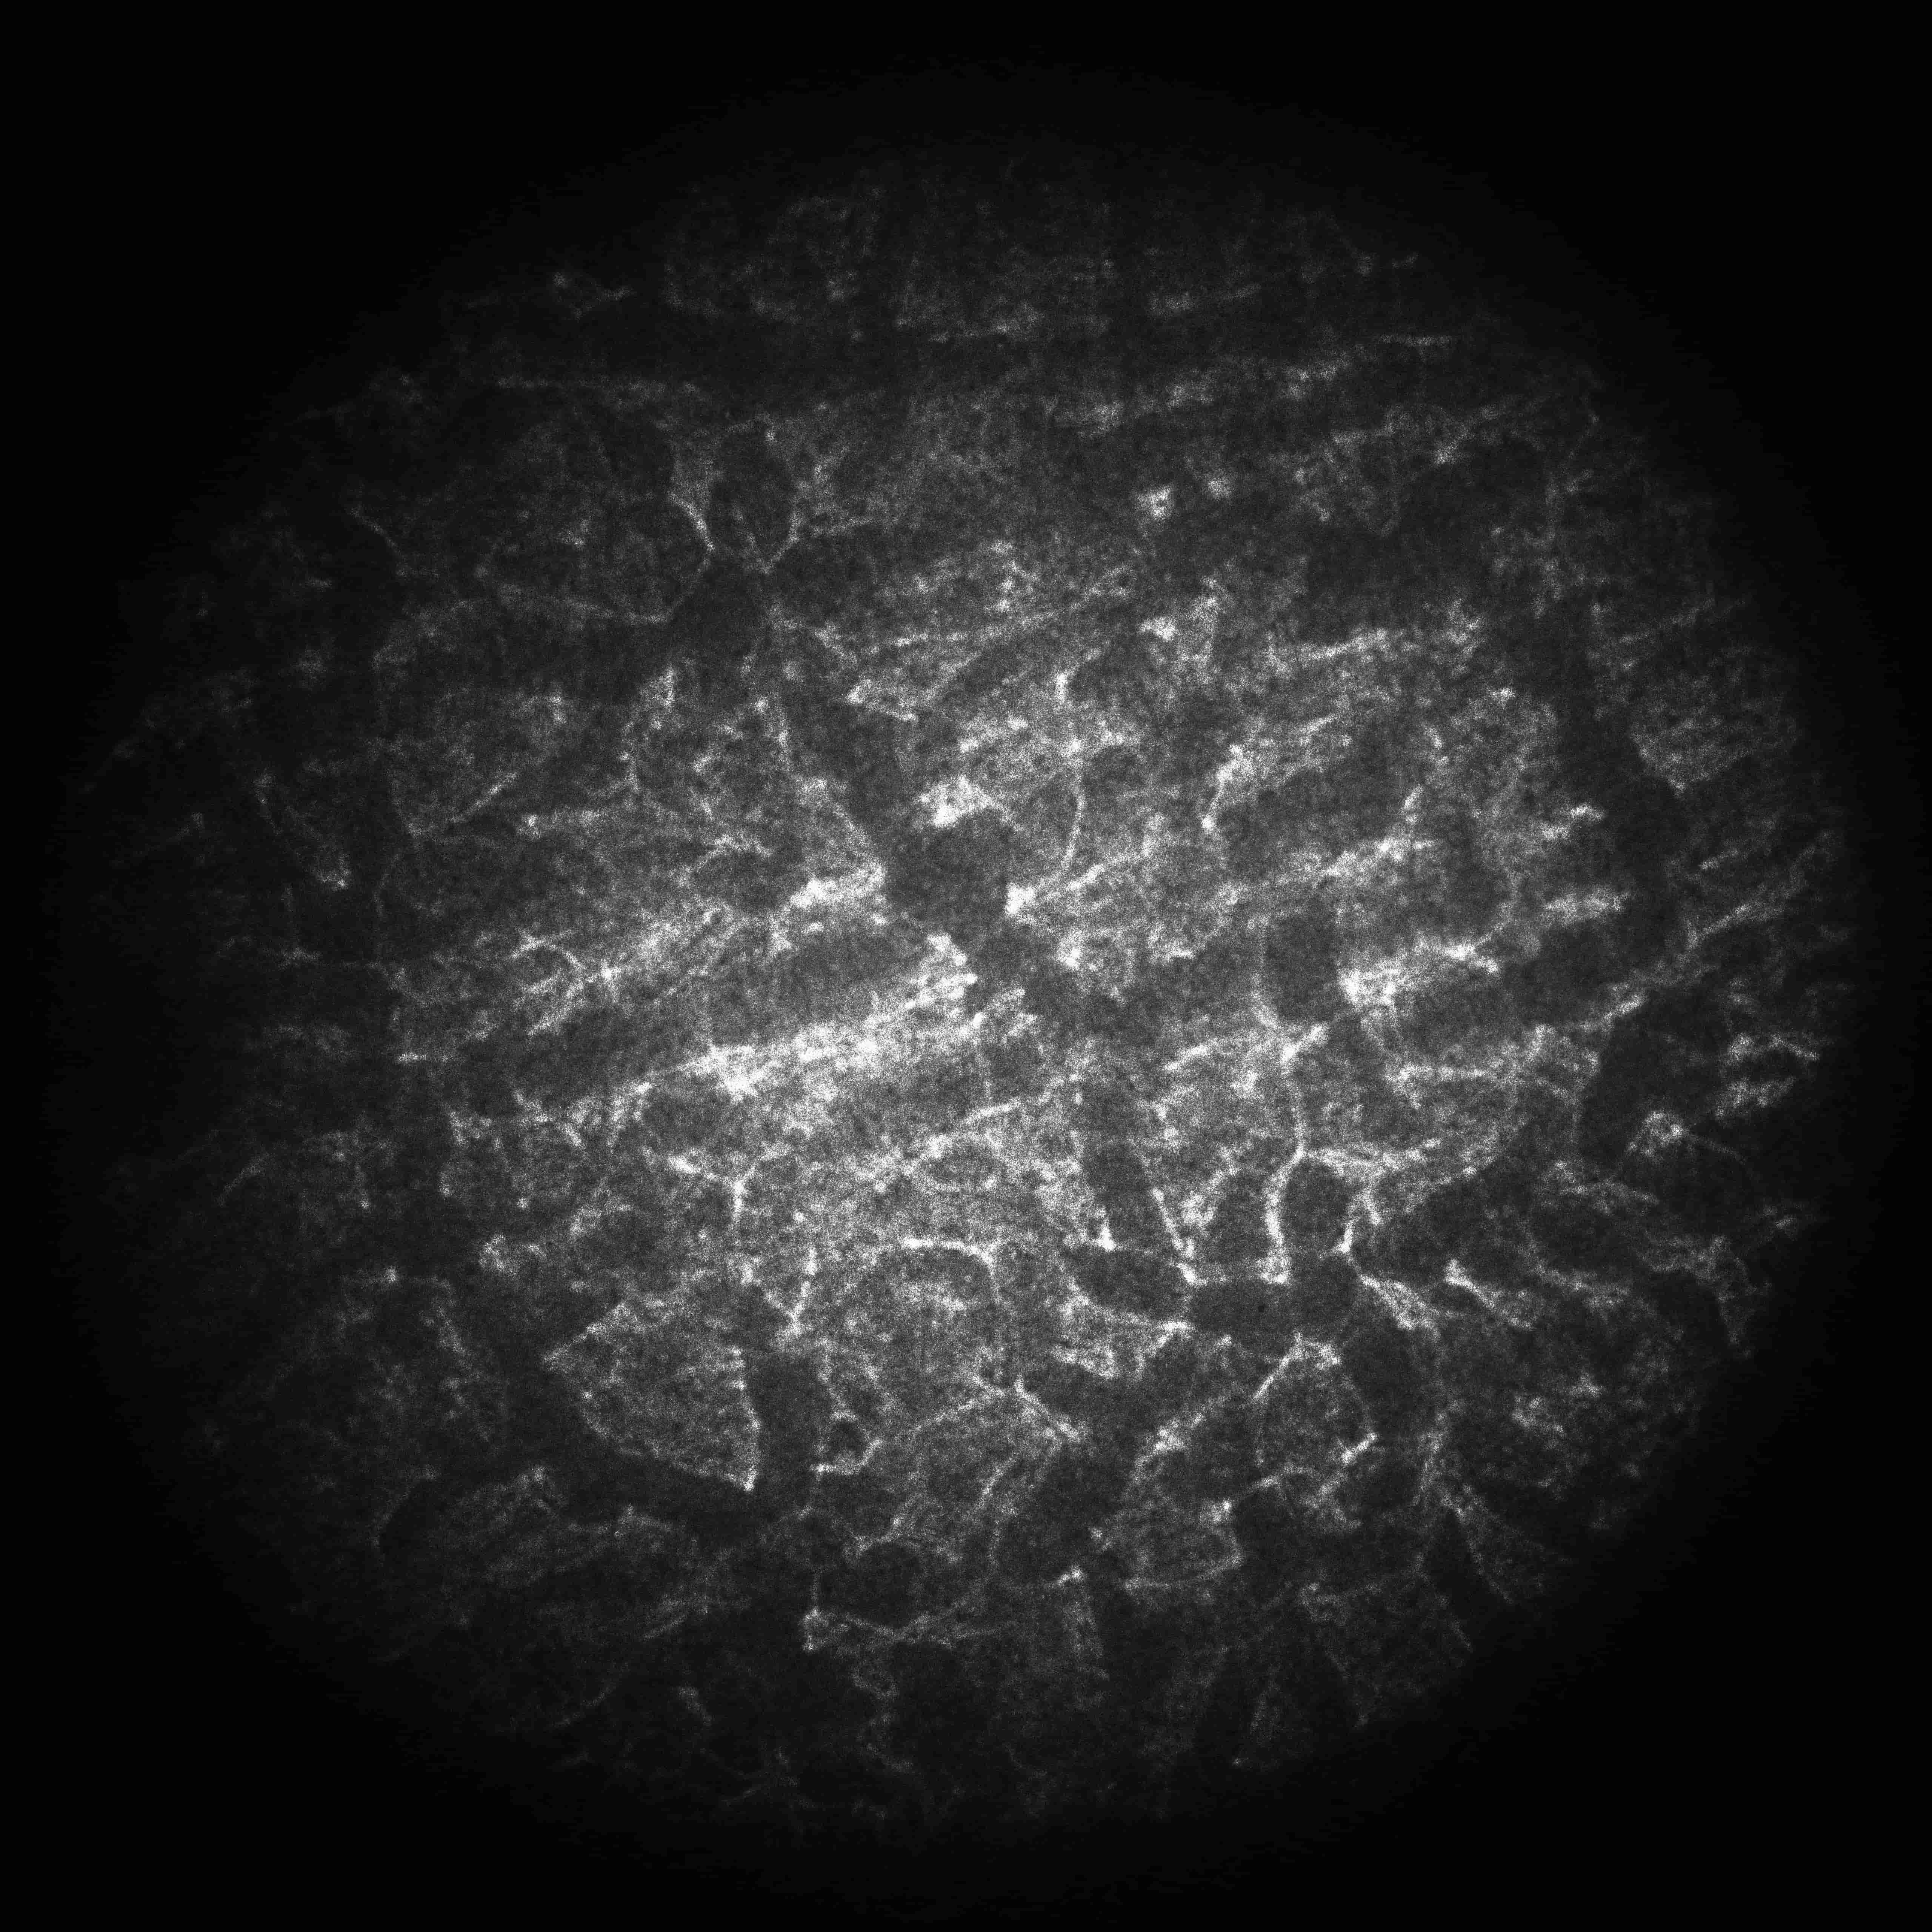
\includegraphics[height=0.3\textwidth]{fig/convection_photos/4mm_1793.jpg}}
    \caption{不同温度差下CCD拍摄得到的斑图。水层厚度$d=4$ mm。}
    \label{fig:convection_photos_4mm}
\end{figure}

之后我们将对流层的厚度改为$d=4$ mm。从\autoref{fig:convection_photos_4mm} 中我们可以看到,水层的增厚会使得临界温度减小,这也符合我们的理论预测:由$Ra\propto d^3\Delta T$和临界条件$Ra=R_c$,可见临界温度差随着$d$的增大而减小,并且呈现三次方反比的关系。但实际上,我们在实验中观察的临界温度为$\Delta T=4.8\ ^\circ\text{C}$(\autoref{fig:convection_photos_4mm}(b)),比我们理论预测值要大。这里给出两个可能的原因:1. 上面$Ra\propto d^3\Delta T$是我们在两个无限大平板之间的系统中推导出来的,而实际上我们的系统是有边界的;2. 我们用CCD图像判断临界点的方法具有一定主观性,只有当我们能在图像中发现可分辨的条纹时,我们才认为系统进入了有序状态,但实际上在我们观察到可分辨的条纹之间,系统就已经达到了临界状态。

在\autoref{fig:convection_photos_4mm}(b) 中我们能够隐约看到圆对称的斑图,但之后随着温度差的增大,圆对称斑图的构型逐渐崩溃,直到\autoref{fig:convection_photos_4mm}(e)(f) 系统进入湍流状态,斑图变得不再稳定。直观上,由于$z$方向范围增大,微扰产生的形式也会更加复杂,这导致了会出现更多的非线性效应,从而更容易导致耗散结构的破坏。

有趣的是,我们在实验中能够观察到\autoref{fig:convection_photos_4mm}(d) 出现了类似于分形结构的斑图。而随着温度差的升高,这样的分形结构会逐渐消失。这里分形的出现绝对不是偶然,虽然我们现在还没有发展出一个很好的理论来解释这个图像出现的原因,但我们可以直观解释分形出现在这里的合理性:分形的自相似性使得分形能够最大化或者最小化某个物理量。例如自然界中树枝的分形结构使得其能够最大程度的吸收阳光,人体中分形的肺泡结构使得氧气能够最大程度的被吸收。因此在我们的实验中,分形结构的出现可能是为了最大程度的增加热量的传输,使得系统能够更快的达到稳定状态。

\section{结论}
本实验通过阴影法观察到了瑞利-贝纳对流斑图的形成和演化,发现了系统的临界点和非线性对流的特征。我们比较了2 mm和4 mm厚度的水层产生的对流,发现随着对流层厚度的增加,系统的临界温度差会减小,而且系统的斑图会变得更加复杂,最终进入湍流状态。虽然在实验过程中由于初始条件没有控制好导致没有能够找到完美的圆对称斑图,但我们还是能够定性认识到系统的演化过程,认识耗散结构的基本特征。

\section{致谢}
感谢周路群老师的悉心指导,尤其是关于耗散结构、非线性动力学以及对实验中许多细节的讲解给本人带来许多启发。这是本人第一次在实验上接触耗散结构的概念,也是第一次体验到耗散结构和非线性系统对于我们所在世界的重要性,这对我来说是一次非常有意义的实验。

\appendix

\section{思考题}
\subsection{随着温差的升高,可以看到黑白结构(即斑图)的出现,黑白的区域如何对应水层的流动情况?}
斑图中黑色的部分为冷水下沉,白色的部分为热水上升,而黑白相间的部分就是一个对流元胞,代表一个完整的对流循环(如\autoref{fig:convection} 所示)。这是因为在室温下,水的密度随温度的升高而降低,从而水的折射率也随温度的升高而降低。根据费马原理,光有向着高折射率介质传播的趋势,因此光会更多的汇聚到温度较低的水的区域,从而在冷水下沉的地方形成较亮的白色区域。由此,我们就可以通过CCD得到的二维图像来反推三维空间中的对流情况。

\subsection{斑图出现的临界点如何确定?如何根据所观察的现象确定临界点?}
当我们能够在CCD图像中看到可分辨的黑白条纹的时候,说明系统到达了临界点。当系统达到从无序到有序的临界点后,系统会重新稳定,因此我们观察到的条纹几乎不会随时间变化,这样的斑图也不会因为小扰动而消失。

\subsection{当水层换成4 mm时,考虑临界点会如何改变?}
因为$Ra\propto d^3\Delta T$,所以当水层从2 mm换成4 mm时,理论上临界温度差是原来的1/8倍。但是实验过程中,临界点的变化并不会这么大,不过定性上临界温度差依然会随着水层厚度的增加而减小。

\subsection{如何确定斑图的空间特征尺度?}
在系统处于稳定状态的时候,CCD中的图像是一个个同心圆(或者近似为同心圆),我们可以通过对这些同心圆的半径进行拟合,从而得到斑图的空间特征尺度。

\subsection{斑图的空间特征尺度与对流水厚度的关系如何?}
斑图的空间特征尺度与对流水厚度成正比。这是因为对流水层的厚度增加,会使得对流元胞的尺度也增大,从而使得斑图的空间特征尺度也增大。斑图的水平尺寸大致和对流水厚度成正比。

\end{document}
